% Document Class
\documentclass{book}

% Define Variables
\newcommand{\gbeauthor}{Pierre-Luc Gagné}

% When to Break Words
\hyphenation{Nin-ten-do}
\hyphenation{Mi-ya-mo-to}

% Table Package
\usepackage[table]{xcolor}
\usepackage{tabulary}

% Createspace: createspace.com/Products/Book/InteriorPDF.jsp
% Geometry: texdoc.net/texmf-dist/doc/latex/geometry/geometry.pdf
\usepackage[
paperwidth=5.5in,
paperheight=8.5in,
top=1.5cm,
headheight=3.5mm,
headsep=6mm,
bottom=1.8cm,
footskip=10mm,
inner=2.29cm,
outer=1.52cm,
marginparsep=0cm,
marginparwidth=0cm
]{geometry}

% Fonts Fonts Fonts !
\usepackage{fontspec}
\setmainfont{Adobe Caslon Pro}
\newfontfamily\pageonegbfont[
  SizeFeatures={Size=28}]
  {Early GameBoy}
\newfontfamily\pageoneauthorfont[
  SizeFeatures={Size=20}]
  {Georgia Italic}
\newfontfamily\footerpokefont[
  SizeFeatures={Size=8}]
  {Pokemon GB}
\newfontfamily\pagetwodescription
  {Avenir Next}
\newfontfamily\titlefont[
  SizeFeatures={Size=30}]
  {Avenir Next Ultra Light}
\newfontfamily\htwofont[
  SizeFeatures={Size=20}]
  {Avenir Next Ultra Light}
\newfontfamily\hthreefont[
  SizeFeatures={Size=14}]
  {Avenir Next Demi Bold}
\newfontfamily\codeintextfont[
  SizeFeatures={Size=12}]
  {Inconsolata}
\newfontfamily\dedication[
  SizeFeatures={Size=12}]
  {Georgia Italic}
\newfontfamily\thisgoesintoc[
  SizeFeatures={Size=14}]
  {Avenir Next}

% Left-Align with \begin{flushleft} and \end{flushleft}
\usepackage{ragged2e}
% Line Spacing with \setstretch{1.1}
\usepackage{setspace}
%Hyphenation control
\usepackage{hyphenat}
% Turn off more space after sentences
\frenchspacing
% Have images align to top by default
\raggedbottom
% Set space between paragraphs
\usepackage{parskip}
\setlength{\parskip}{0.8em}
\setlength{\parindent}{1.5em}

% Image Package
\usepackage{graphicx}
\usepackage{float}
\graphicspath{ {book-assets/} }
\usepackage{wrapfig}
\usepackage{adjustbox}
\usepackage{placeins}

% List item package
\usepackage{enumitem}

\let\oldcenter\center
\let\oldendcenter\endcenter
\renewenvironment{center}{\setlength\topsep{0pt}\oldcenter}{\oldendcenter}

% Page Details
% Show wireframes for development
%\usepackage{showframe}

% Define Chapters
\usepackage{needspace}
\usepackage{titlesec}
\titleformat{name=\chapter}[block]{\titlefont\raggedright\setstretch{3}}{}{0pt}{}[]
\titlespacing{name=\chapter}{0pt}{-30pt}{6pt}[0pt]
\titleformat{name=\section}[block]{\htwofont\raggedright\setstretch{2}}{}{0pt}{}[]
\titlespacing*{name=\section}{0pt}{10pt}{0.4em}[0pt]
\titleformat{name=\subsection}[block]{\hthreefont\raggedright\setstretch{1.8}}{}{0pt}{}[]
\titlespacing*{name=\subsection}{0pt}{4pt}{0.4em}[0pt]

% Table of Contents
\usepackage{titletoc}
\renewcommand{\contentsname}{Table of Contents}
\titlecontents{chapter}[0pt]{\thisgoesintoc}
{\thecontentslabel\enspace}
{}
{\titlerule*[4pt]{.}\raggedright\contentspage}[\vskip 7pt]

% Headers & Footers
\usepackage{fancyhdr}
\fancyhf{} % sets both header and footer to nothing
\renewcommand{\headrulewidth}{0pt}
\pagestyle{fancy}
\renewcommand{\chaptermark}[1]{\markboth{#1}{}}
\lhead[]{}
\chead[]{}
\rhead[]{}
\lfoot[\footerpokefont \thepage]{\pagetwodescription \leftmark}
\cfoot[]{}
\rfoot[]{\footerpokefont \thepage}

\fancypagestyle{plain}{
\fancyhf{}
\fancyfoot[R]{\footerpokefont \thepage}}

% Making printing compliant PDF
%\usepackage[x-1a]{pdfx}

% Begin Document
\begin{document}
\begingroup
\setlength{\columnsep}{1.7mm}
\setlength{\intextsep}{0mm}

\thispagestyle{empty}
\mbox{}
\vskip 70pt
\begin{flushleft}
\setstretch{4}
\pageonegbfont \nohyphens{\gbetitle{} \par}
\setstretch{3}
\pageoneauthorfont \nohyphens{by \gbeauthor{} \par}
\end{flushleft}
\vfill
\newpage

\thispagestyle{empty}
\mbox{}
\vfill
\begin{center}
\setstretch{1}
\fontsize{10pt}{12pt}\selectfont
\pagetwodescription {\gbetitle{}\par © \gbepublishedyear{} by Pierre-Luc Gagné\par \vskip 9pt gameboyessentials.com \vskip 9pt \gbeeditionname{}\par \vskip 9pt This book is set in Adobe Caslon Pro, with Inconsolata for monospaced segments, and Avenir Next for headings. It also uses fonts from {\em Super Mario Land} and {\em Pokémon} for flourishes. \vskip 9pt ISBN \gbeISBN{}\par \vskip 9pt The copyright for game boxes and screenshots reproduced in this book remain with the respective owners of those works.}
\end{center}
\newpage

\thispagestyle{empty}
\mbox{}
\vfill
\begin{raggedleft}
\setstretch{1.1}
\dedication{\gbededication{}}
\vfill
\end{raggedleft}
\newpage

\begingroup
\let\cleardoublepage\clearpage
\tableofcontents
\endgroup
\thispagestyle{empty}
\fontspec{Adobe Caslon Pro}[WordSpace = 1.1]
%\fontspec{Adobe Caslon Pro}
%\addfontfeature{LetterSpace=1.0}
\setstretch{1.2}
\fontsize{12pt}{12pt}\selectfont











































































\begingroup \chapter*{Game Boy Camera}\markboth{Game Boy Camera}{}\addcontentsline{toc}{chapter}{Game Boy Camera} \endgroup
\begin{figure}[H]
\vskip 4pt
\centering
\includegraphics[width=.75\linewidth]{assets/assets/mgb-006/mgb-006-1.jpg}\end{figure}
\begin{itemize} [nosep]




\item Japanese release in February 1998
\begin{itemize} [nosep]\item Clear Purple\end{itemize}\noindent






\item Japanese release in February 1998
\begin{itemize} [nosep]\item Green\end{itemize}\noindent






\item North American release in June 1998







\item European release in 1998












\item Developed by Nintendo

\end{itemize}\noindent

\newpage\FloatBarrier\needspace{10mm}\section*{A Camera in Your Pocket}\nopagebreak[4]
\begin{wrapfigure}{L}{0pt} \includegraphics[width=.45\linewidth]{assets/assets/mgb-006/mgb-006-2.png}\end{wrapfigure}
Where is the closest camera you own right now? In your pockets? If you’re reading this on your phone, you have a camera looking at you right now, and a whole family of high-quality sensors on the back of the very device with which you’re reading this article. The ubiquity of cameras has thoroughly changed our society, from personal communications to police oversight. The Game Boy Camera came out at a time well before that revolution when a photograph was still an event. The closest peer to this accessory in terms of size and price in 1998 were disposable cameras. Costing \$10 or lower, disposable cameras were a democratizing force for the camera world. They allowed you to enjoy photography for a very small initial investment. However, they did not change the fundamentals of film cameras; you needed to pay for film development for all the pictures you took, even for duds you were going to throw away.

Digital cameras were already available in 1998. With their rewritable media, they allowed you to take and delete an infinite number of pictures. You were limited only by your digital storage space. In 1998 most cameras saved their pictures on 3 \& 1/2-inch diskettes, which meant you could carry a stack of them with you. However, the Sony Mavicas sold for around USD \$800 at that time; an expensive sum for very low-resolution pictures. The Game Boy Camera is a peer of those early digital cameras. It was unique amongst digital cameras for its very low price, which came with absurd limitations that severely limited its appeal. We’ll discuss this fascinating Nintendo device in detail, and together we’ll discover what motivated the employees at Nintendo to make the Game Boy Camera.

\FloatBarrier\needspace{10mm}\section*{A Greyscale Camera}\nopagebreak[4]

\begin{quote}When Gunpei Yokoi left Nintendo, Hirokazu Tanaka felt betrayed by his departure, and wanted to prove that people at Nintendo could still apply his lessons to create inventive products. The Game Boy Camera and its printer were born of this desire to show the creativity of the developers who stayed with Nintendo. Yokoi accidentally died before the camera was released, and his thanked in the credits.\newline \emph{—Translated from \emph{L’histoire de Nintendo Volume 4}, P. 153.}\end{quote} \par

Gunpei Yokoi is best remembered as the father of the Game Boy, since he was the leader of R\&D1 where the device was developed. When Yokoi left Nintendo in the mid ’90s, Hirokazu \emph{Hip} Tanaka, a music composer inside the company, saw the Game Boy Camera project as a way to prove his and his colleagues’ worth. They had the engineers to develop future iterations of the Game Boy, but they had lost their superstar toymaker. Yokoi was famous for his work at Nintendo; a rare privilege only bestowed back then upon him and Shigeru Miyamoto. Miyamoto was a video game developer but Yokoi was something else entirely. He was an engineer and an inveterate tinkerer. Ultimately, he was Nintendo’s star toymaker. Yokoi had started at Nintendo when it was still a playing card company, and his wonderful designs gave Nintendo a solid footing when it diverted in toymaking. The stories around Yokoi’s mechanical creations were legend. With Yokoi’s departure, the R\&D1 division was further divided into a hardware and a software section. Okada Satoru was put in charge of the hardware, and no one internally could doubt his ability to deliver good products, since he was the person who defined all the important details of the Game Boy. An engineer who started at R\&D1 working for Yokoi, he went against his boss during the Game Boy’s development. Yokoi wanted the Game Boy to be similar to a Game \& Watch that would be popular for a \emph{season}. Perhaps a machine that could only play a limited set of predetermined games. Yokoi had the mentality of a toy-maker; he focused on building toys that would grab children’s attention for a moment before they moved on to something else. It was Okada that wanted a hardware platform that developers could fully program. Something where our waning attention is focused on the cartridges, not on the hardware. Simply put, a portable Famicom. Yokoi relented and let Okada build the Game Boy his way. This highlights the trustworthiness and competence of Okada; he would continue to deliver portable success after portable success until his retirement from Nintendo in 2012. Back in 1998, he had not yet proven himself, and was certainly not known for his toymaker mentality. Making a digital camera for the Game Boy might prove that Nintendo R\&D1 could still make interesting toy-like accessories without Yokoi.

\FloatBarrier\needspace{10mm}\section*{Limited Hardware}\nopagebreak[4]

With our modern point of view, \emph{Game Boy Camera} is a complete joke. It can seem like no one could tolerate its low image quality and that it must have been a monumental flop. The reality is far from that. Looking back at the \emph{Game Boy Camera}’s release in 1998, the device enjoyed a somewhat warm reception.

\begin{figure}[hbt]
\vskip 10pt
\centering \includegraphics[width=.75\linewidth]{assets/assets/mgb-006/mgb-006-3.jpg}\par\pagetwodescription Popular Science, July 1998, p. 12
\vskip 6pt
\end{figure}
\begin{figure}[hbt]
\vskip 10pt
\centering \includegraphics[width=.75\linewidth]{assets/assets/mgb-006/mgb-006-4.jpg}\par\pagetwodescription Boys’ Life, September 1998, p. 11
\vskip 6pt
\end{figure}
\begin{figure}[hbt]
\vskip 10pt
\centering \includegraphics[width=.75\linewidth]{assets/assets/mgb-006/mgb-006-5.jpg}\par\pagetwodescription Vibe, August 1998, p. 148
\vskip 6pt
\end{figure}
\begin{figure}[hbt]
\vskip 10pt
\centering \includegraphics[width=.75\linewidth]{assets/assets/mgb-006/mgb-006-6.jpg}\par\pagetwodescription GamePro, August 1998, p. 30
\vskip 6pt
\end{figure}

Yes, the pictures it takes are laughably bad, with a ridiculously low 128 by 112-pixel resolution. The thing is only good at taking pictures of large things (like a head or a dog) from way up close. Don’t even try to take a picture of a distant landscape view. To top off the mediocrity, pictures have no colour, being only available in the same four shades as your Game Boy. However, you have to look at what digital cameras were capable of doing and at what price to understand the device’s appeal in 1998. Of course, something like the Canon EOS D2000 existed, but this 1728 by 1152 resolution professional device retailed for over \$15,000 USD. It was also a bleeding edge trailblazer; it was the first digital camera somewhat respected by professionals. We have to look downmarket to find peers of our little puny \emph{Game Boy Camera}. For example, Minton made a crappy OEM camera that was re-badged by countless companies. It came with a 640 x 480 pixel sensor and sold for around \$149 USD. It’s a much better device at three times the price but it is still a terrible camera compared to modern standards.

When you look at it, the Game Boy Camera is more akin to a toy than a digital camera. We’re lucky, we have a new camera toy from 1998 to compare it against.

\begin{figure}[hbt]
\vskip 10pt
\centering \includegraphics[width=.75\linewidth]{assets/assets/mgb-006/mgb-006-7.jpg}\par\pagetwodescription BarbieCam!
\vskip 6pt
\end{figure}

\emph{Barbie Photo Designer} was announced in September of 1998, obviously for the upcoming Holiday season and was a package consisting of the digital camera and its accompanying PC software. It retailed for \$69.99, a shockingly low price at first glance for a digital camera and PC software. Upon closer examination the device is not too good to be true. Although it took colour photos, it is very close to the Game Boy Camera in terms of resolution: 160 by 120 pixels. That’s minuscule.

\begin{figure}[hbt]
\vskip 10pt
\centering \includegraphics[width=.75\linewidth]{assets/assets/mgb-006/mgb-006-8.jpg}\par\pagetwodescription An example of a BarbieCam photo. This photo was taken with the later Nickelodeon model, which is the same camera. Photo courtesy of Superkids.com.
\vskip 6pt
\end{figure}

It was a severely limited device. It’s a digital camera but it doesn’t have a screen or removable media. All the beautiful benefits of digital photography come from those two things. Without a screen you can’t know if the picture you took is any good and without removable media you can’t keep taking pictures by swapping SD cards or whatnot. You’re stuck with the six pictures it can keep in its internal memory.

The device’s only options are taking pictures or deleting all the meagre six pictures without ever looking at them. Once you connect to a PC, you can very slowly transfer your pictures and finally see them for the first time. I imagine most kids ended up using the device in their home fairly close to their PC due to those extreme limitations.

Moving on to the software, both companies chose to focus on offering games with the pictures you took to complement their low-resolution cameras. I guess there aren’t many ways to make a bad quality camera \emph{fun}. When you compare the disadvantages of \emph{Barbie Photo Designer} and \emph{Game Boy Camera}, that’s where you understand that the portability, viewfinder and memory for 30 pictures make the \emph{Game Boy Camera} a competitive package in this brand new toy camera category. This category was hotter than you think as well: \emph{Barbie Photo Designer} sold 300,000 copies in the US in its first year on the market and the \emph{Game Boy Camera} sold a million copies in Japan. However, the market would quickly get saturated with copycats, and by the mid-2000s digital cameras had come down in price enough that a toy digital camera became a niche item. Parents seemingly bought their kids cheap full-fledged cameras instead.

\FloatBarrier\needspace{10mm}\section*{Terrible Software}\nopagebreak[4]

I’ll say it upfront; I don’t like the \emph{Game Boy Camera} software. It’s a mess. It features so many baffling interface decisions. People have called it quirky. I have a different word for it: bad.

\begin{figure}[hbt]
\vskip 10pt
\centering 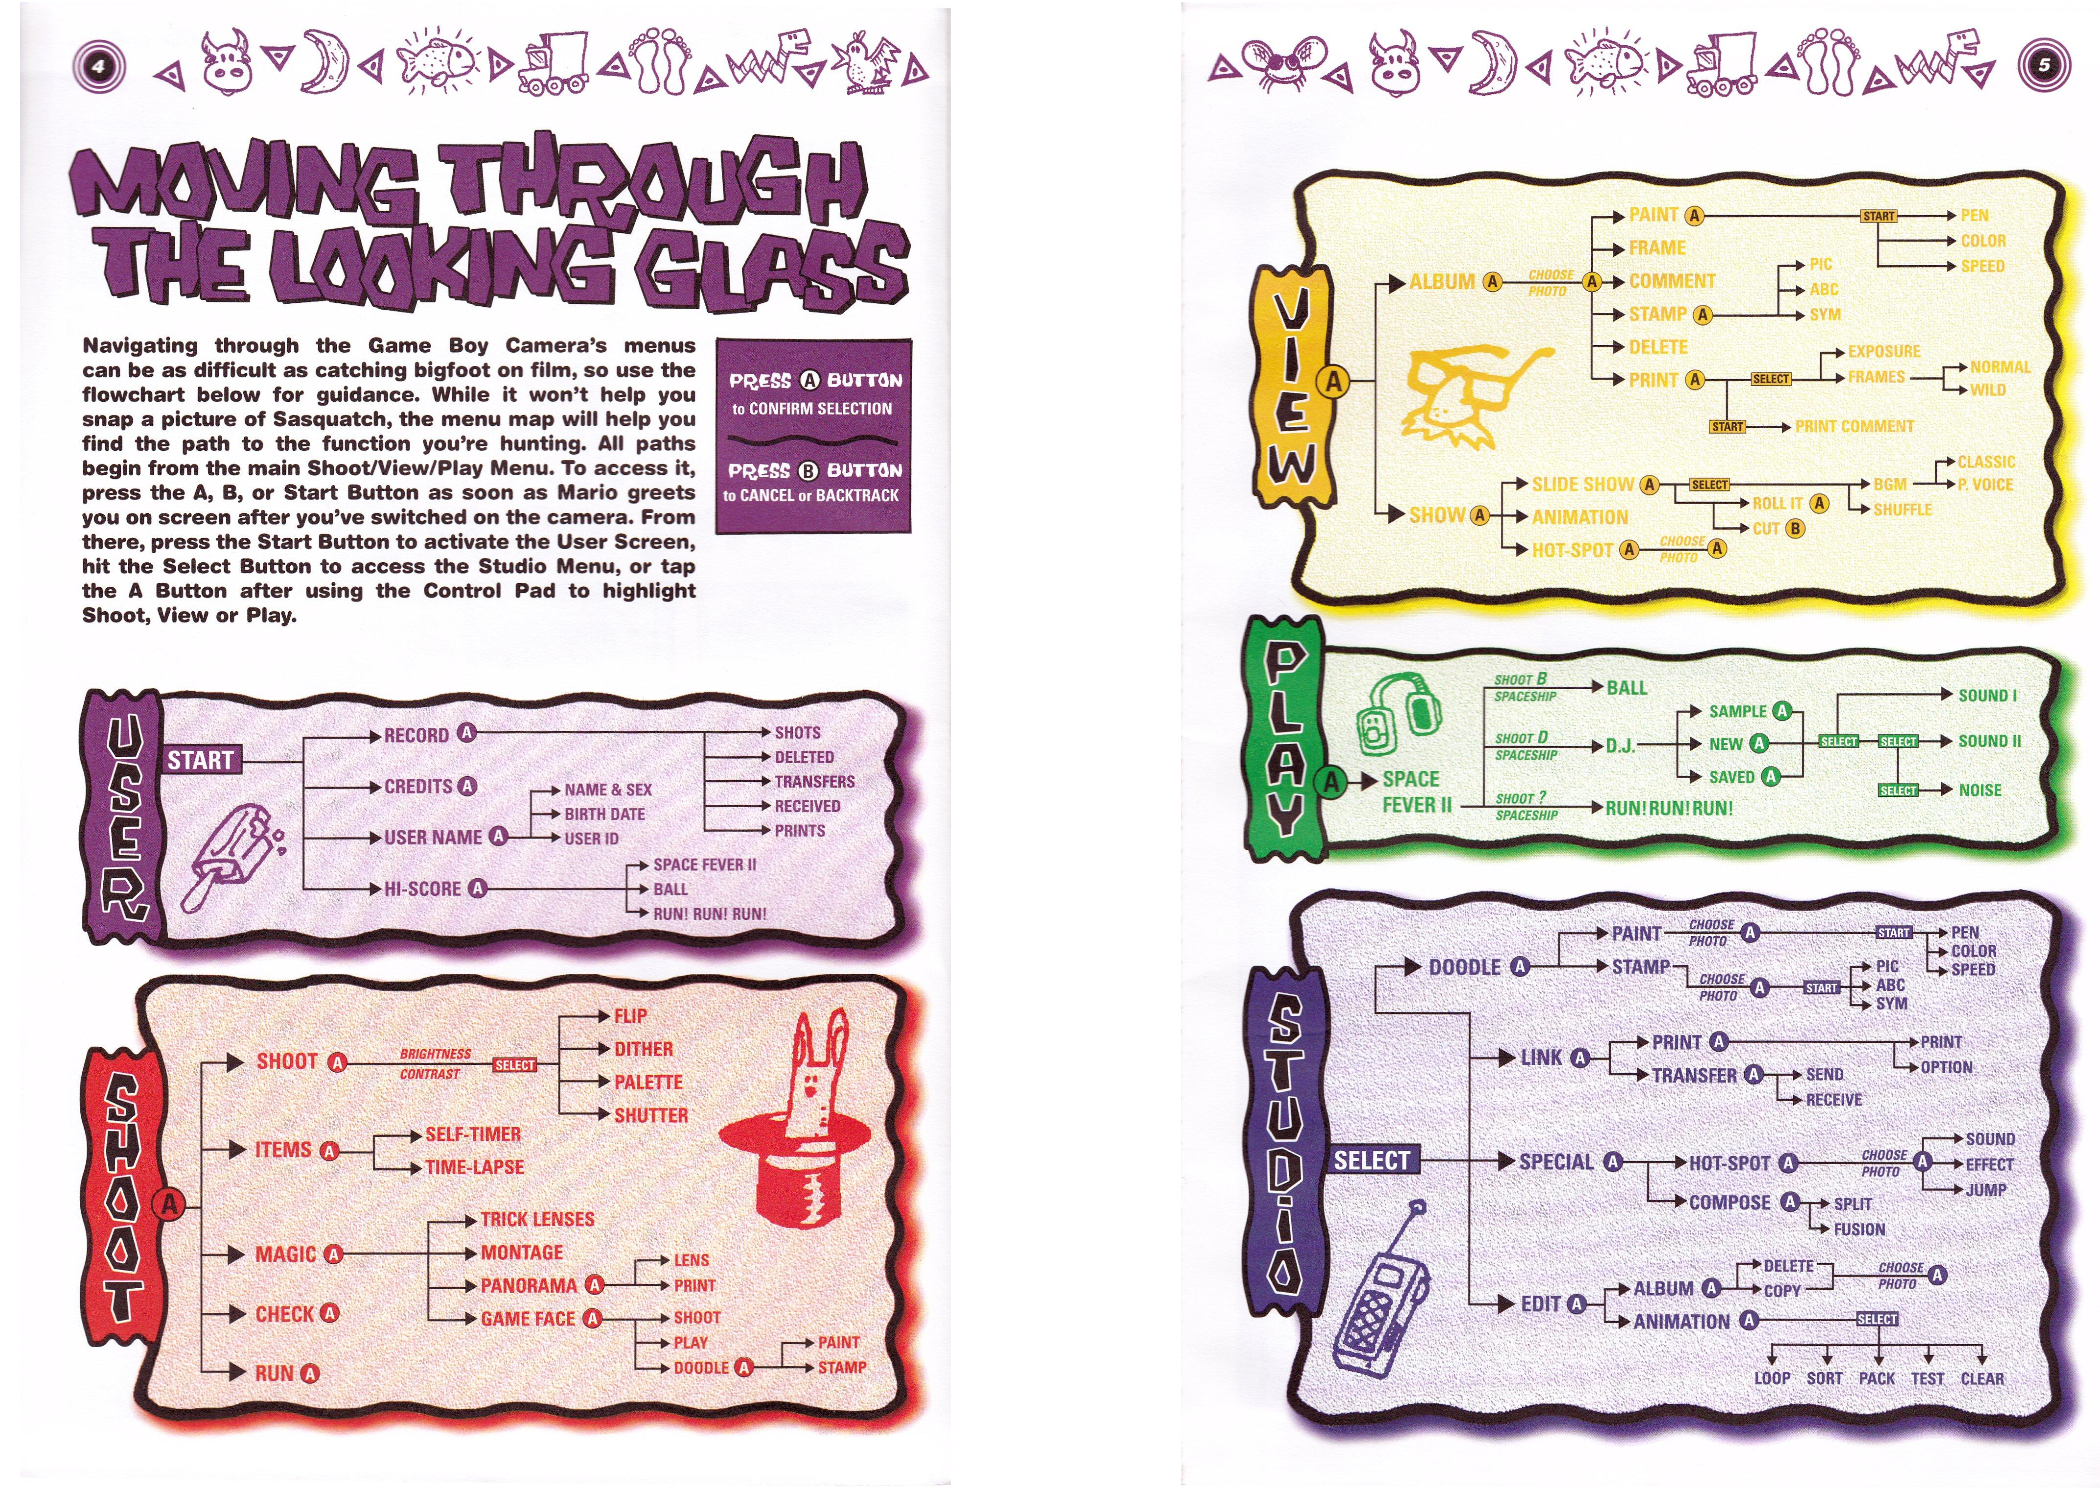
\includegraphics[width=.75\linewidth]{assets/assets/mgb-006/mgb-006-9.jpg}\par\pagetwodescription The Nintendo Game Boy Camera Funtography Guide provides a full map of the software.
\vskip 6pt
\end{figure}

You can immediately see that there are a lot of things you can do. Outside of \emph{Mario Paint}, I can’t think Nintendo had ever made a user interface this complex before.

Upon starting the device, you’re presented with a start screen with photos of someone in a Mario costume. This shows one conceit of the software; that it will sometimes use real photos taken with a \emph{Game Boy Camera}. It’s not a full design choice. Large sections of the interface use drawn art to represent characters. If you get an idea like that, I’d expect them to use it fully.

\begin{wrapfigure}{L}{0pt} \includegraphics[width=.45\linewidth]{assets/assets/mgb-006/mgb-006-10.png}\end{wrapfigure}

We get a complete rookie mistake on the main screen of the interface: they never indicate you can press the Start button to access settings. So on a screen with three clearly written choices, you actually have four. Let’s jump into the worst segment of the device; Play. When you go into this segment, a game of \emph{Space Fever II} immediately begins. Two enemies drop down from the top of the screen, with letters written on them. Now, those enemies are actually the selection method for the \textbf{other} games you can play. So if you shoot those lettered enemies, you start another completely different game. However, if you shoot none of them, or miss your shot, \emph{Space Fever II} will begin. Imagine that; a selection menu with a time limit. Upon starting those other games, you get astoundingly different screens to navigate their respective options. There is no general logic. The whole UI is a mad house.

\begin{center}
\vspace{8pt}\adjustbox{valign=t}{\includegraphics[width=.45\linewidth]{assets/assets/mgb-006/mgb-006-11.png}}
\quad\vspace{4pt}\adjustbox{valign=t}{\includegraphics[width=.45\linewidth]{assets/assets/mgb-006/mgb-006-12.png}}
\quad\vspace{4pt}\adjustbox{valign=t}{\includegraphics[width=.45\linewidth]{assets/assets/mgb-006/mgb-006-13.png}}
\end{center}

The first game is a copy of the first Game \& Watch title, \emph{Ball}. We’ve discussed it previously when talking about \emph{Game Boy Gallery}. This version is using different sprites for the body, and allows you to use pictures for the face. The second game is a small DJ toy that I cannot understand for the life of me. The final game, which you unlock upon completing \emph{Space Fever II}, is a running game where you mash buttons. Once again, you can put your face on the character you play.

\begin{figure}[hbt]
\vskip 10pt
\centering \includegraphics[width=4.85cm]{assets/assets/mgb-006/mgb-006-14.png}\par\pagetwodescription The Shoot menu
\vskip 6pt
\end{figure}

Upon going to the Shoot segment, you get what is supposed to be a parody of an RPG’s battle screen, with pixel art of people standing in as your enemies. Since you just came from a screen where someone in a Mario suit was dancing about, the joke falls flat immediately. The battle screen includes a run command, leading to an infamous joke played on the user.

\begin{figure}[hbt]
\vskip 10pt
\centering \includegraphics[width=4.85cm]{assets/assets/mgb-006/mgb-006-15.png}\par\pagetwodescription What are you running away from? BAD UI!
\vskip 6pt
\end{figure}

That jokey screen is meant to tell the player that they can’t run away, this isn’t an RPG, just a parody of one. But the very real face has those hideous drawings added on them. It’s just so out of place.

The two most sedate and reasonable segments of the software are the viewfinder screens and the photo album under View. The picture taking features all the controls around the viewfinder, arranged in an intelligent manner that focuses on quick adjustments. The photo album navigation is pretty straightforward, and once you reach the single picture view, all the options are also arranged around the picture. If you dig deep enough, you can find drawing tools that provide you with a barebones \emph{Mario Paint}. You could take a picture of a white wall and just draw on your Game Boy. You don’t get the benefit of a mouse, but it’s a fun, well designed little drawing utility in a sea of terrible UI.

\begin{center}
\vspace{8pt}\adjustbox{valign=t}{\includegraphics[width=.45\linewidth]{assets/assets/mgb-006/mgb-006-16.png}}
\quad\vspace{4pt}\adjustbox{valign=t}{\includegraphics[width=.45\linewidth]{assets/assets/mgb-006/mgb-006-17.png}}
\quad\vspace{4pt}\adjustbox{valign=t}{\includegraphics[width=.45\linewidth]{assets/assets/mgb-006/mgb-006-18.png}}
\quad\vspace{4pt}\adjustbox{valign=t}{\includegraphics[width=.45\linewidth]{assets/assets/mgb-006/mgb-006-19.png}}
\quad\vspace{4pt}\adjustbox{valign=t}{\includegraphics[width=.45\linewidth]{assets/assets/mgb-006/mgb-006-20.png}}
\quad\vspace{4pt}\adjustbox{valign=t}{\includegraphics[width=.45\linewidth]{assets/assets/mgb-006/mgb-006-21.png}}
\end{center}

The camera has far more tricks up its sleeve, and they are all bespoke tools that are hard to grasp because their user interface is not standardized. All in all I think part of the mess is explained by the number of companies who worked on the project. Employees from Creatures (formerly Ape), Game Freak, and R\&D1 are all credited. This is a complete guess, but I think employees completed different segments of the software alone and those were added together with no regards for consistency. Even Jupiter, the company mostly known for Picross, is thanked in the credits but they might have supported in other ways like Quality Assurance. None of the craziness in the software was featured on the box; the box is very sedate, even in Japanese. The ads themselves, in both Japan and the US, focus heavily on the power of easy photography (duh) and the fun that can be had with the stamps implemented in the painting tools of the photo album.

\begin{center}
\vspace{8pt}\adjustbox{valign=t}{\includegraphics[width=.45\linewidth]{assets/assets/mgb-006/mgb-006-22.png}}
\quad\vspace{4pt}\adjustbox{valign=t}{\includegraphics[width=.45\linewidth]{assets/assets/mgb-006/mgb-006-23.png}}
\end{center}

We got a surprising revelation just recently in 2020 that highlights the poor user interface design. As a part of the \emph{Gigaleak}, a massive lotcheck of Game Boy titles was uncovered. Lotchecks, in internal Nintendo parlance, are lists of ROM ready for use in cartridges. They’re the golden masters. Amongst this lotcheck was \emph{Hello Kitty Pocket Camera}, a special version of the camera dedicated to whom else but Hello Kitty. This whole special version of the Game Boy Camera is 100\% complete, yet was \textbf{never released}. No one outside Nintendo had seen this software before 2020. When you load up this golden master in an emulator you can see all the beautiful differences. While all the camera functionality from the released version is present, nothing from the released Game Boy Camera user interface was reused. I’m not versed enough in Japanese to explore the interface in detail but my cursory look revealed a much improved UI. For example, if pressing Start sends you to another screen, you see a mention from the Hello Kitty UI. All the creepy pictures and inscrutable in-jokes have been removed. It’s clear the Hello Kitty UI was their second attempt at a \emph{Game Boy Camera} interface, and this second crack at the problem gave them enough time to finally make a workable interface. It’s just a shame they never released it.

\begin{figure}[hbt]
\vskip 10pt
\centering \includegraphics[width=.75\linewidth]{assets/assets/mgb-006/mgb-006-24.jpg}\par\pagetwodescription We know what the hardware could have looked like from a Pocket Hello Kitty flyer.
\vskip 6pt
\end{figure}

\FloatBarrier\needspace{10mm}\section*{Game Boy Camera Gets a Receipt Printer}\nopagebreak[4]

Nowadays, people are satisfied that their photos live online, but in 1998, everybody expected to get printed copies of every picture they took. You could trade pictures with another \emph{Game Boy Camera} using a Link Cable, but keeping your pictures imprisoned inside a \emph{Game Boy Camera} was a non-starter; Nintendo wanted to provide printing capabilities. While Nintendo could have answered with a stereotypically Japanese solution by putting printing kiosks in combinis all over Japan, leaving the rest of the world to fend for itself, they instead developed a portable printer one could easily buy alongside the camera. This was a great idea in practice, and a marked improvement over \emph{Mario Paint}. I feel like \emph{Mario Paint} never reached its full potential because it never had any print capabilities outside of \emph{record your art on a VHS tape and figure something out from there}.

\begin{figure}[hbt]
\vskip 10pt
\centering \includegraphics[width=.75\linewidth]{assets/assets/mgb-006/mgb-006-25.jpg}\par\pagetwodescription The Game Boy Printer.
\vskip 6pt
\end{figure}

So as with the camera came the Game Boy Printer. Connected through the link cable port, running with a whopping six AA batteries and retailing for the relatively high price of \$60 upon release in 1998, the device uses thermal paper just like your receipt at the grocery store. Just like we discussed earlier with the camera, Nintendo knew they had to compensate for their bargain bin technology, so they wisely included thermal paper with a sticking back. This turned bad pictures into \emph{collectable pictures}. You could stick your pictures in a book, collect pictures of different plants or animals, stick pictures of people on their books, etc. Selling paper with a sticky back was a genius idea to compensate for a poor printing quality; and the printing quality was indeed bad. No one goes to a thermal printer for a beautiful, detailed print. It’s a cheap way to get something on paper fast. It will work fine for fun prints to share in the moment, but you’re not going to preserve your pictures long-term with those prints. Just like your receipts the prints fade with time. So if you have any old printed pictures from way back, they’ll be very faded now, due to the thermal paper technology.

The Game Boy Printer enjoyed a life outside its release with the \emph{Game Boy Camera}. A few games included the ability to print some stuff; banners, high scores, medals. \emph{Pokémon Yellow} allowed you to print the content of your PC boxes for example, providing potential relief from all the box shuffling needed to manage your captured Pokémons. When I look at an exhaustive list of what can be printed, I find nothing impressive. Add the high price of the printer coupled with its large appetite for batteries and I feel like anyone who bought the printer was disappointed by its usage outside of \emph{Game Boy Camera}. I didn’t buy it, and still do not own one; when I bought my \emph{Game Boy Camera}, I did so for \$20, a year after its release in the fall of 1999. I skipped the printer, which still retailed for its full price somehow. I don’t feel like I’m missing anything, especially since the Game Boy Printer is basically a repurposed receipt printer mechanism.

\FloatBarrier\needspace{10mm}\section*{Accessing Your Pictures}\nopagebreak[4]

\begin{wrapfigure}{L}{0pt} \includegraphics[width=.45\linewidth]{assets/assets/mgb-006/mgb-006-26.png}\end{wrapfigure}
If you’re like me, you own a \emph{Game Boy Camera} with pictures that are decades old at this point. You might even have pictures that you consider valuable stuck on there. My sister had taken pictures of our family dog when he was a puppy. I wanted a way to extract them and get copies on my Mac. Having already explained how a Game Boy Printer is a poor fit for preservation, other options were needed.

Five or ten years ago, limited options existed but we now have a plethora of methods to extract pictures from a Game Boy, from the handmade low-run device like the BitBoy to the exquisite FPGA high-quality device like the Analogue Pocket. You also have the Epilogue GB Operator a cartridge port you somehow plug into your computer to play those games, and something like the Game Boy Camera Fast Wifi Adapter a project you assemble yourself using a bunch of parts that you fit inside a 3D printed case. Basically it’s a GBxCart RW coupled with a Raspberry Pi Zero. There are even more options if you want to do a bit of research. To solve the problem for me, I used something I already owned. Since I’m cheap, and didn’t want to spend money on a bespoke solution I’ll use once, I decided to use the little Arduino board I already own to transfer my pictures. This meant cutting up a Game Boy link cable and identifying each wire with continuity. Not the easiest thing, but it was a reasonable task for an amateur tinkerer like me. I was able to adequately mark the required wires, make new ends (always be sure to plug the ground wire in the right spot) and follow the instructions to load the software correctly and extract the data from the serial monitor. It was immediately successful, with my only issue being the extremely crappy software for the Arduino IDE. They should be ashamed of how many interface bugs they have in their software. Anyway, I encourage you to get your pictures extracted if you have any of sentimental value. That cell battery in there won’t last forever.

\begin{figure}[hbt]
\vskip 10pt
\centering \includegraphics[width=4.85cm]{assets/assets/mgb-006/mgb-006-27.png}
\vskip 6pt
\end{figure}

\FloatBarrier\needspace{10mm}\section*{Never the Smallest}\nopagebreak[4]

I had read on Wikipedia that the 1999 edition of the \emph{Guinness Book of World Records} deemed the \emph{Game Boy Camera} the world’s smallest digital camera. I wanted to read this mention in Guinness directly, so I headed to the Internet Archive’s controversial book rental system to read the 1999 Guinness book. Here is the paragraph talking about the Game Boy Camera on page 294.

\begin{figure}[hbt]
\vskip 10pt
\centering \includegraphics[width=.5\linewidth]{assets/assets/mgb-006/mgb-006-28.jpg}
\vskip 6pt
\end{figure}

\begin{quote}
SMALLEST CAMERAS In 1998, Nintendo’s Game Boy, which was launched in 1989 and has sold more than 60 million units worldwide, was reinvented as a camera and printer. The digital still camera cartridge sits on top of the Game Boy (as seen at left) and can take and store up to 30 low-resolution black and white photos. The camera comes with three games that allow players to create characters using photos. The printer can then produce small prints or stickers. In 1997, the company reduced the size of the Game Boy and introduced the Game Boy Pocket, and a color version of the Game Boy is due to be launched at the end of 1998. The world’s smallest pinhole video camera is the PC-21XP, sold by Supercircuits Inc. The CCD element occupies only ¼ square inch but has a 295,000-pixel array that outputs 380 video lines. It can see in low-level lighting of 0.5 lux. The overall unit measures 115/100 × ½ inch and can run for up to five hours on one PP3 battery.
\end{quote} \par

As you can see reading it, no mention is made of the Game Boy being the smallest of anything. You could perhaps read the description of the PC-21XP described as the world’s smallest pinhole video camera and think this applies to the \emph{Game Boy Camera}. Unfortunately, the cartridge does not use a PC-21XP as its camera element. The camera uses a Mitsubishi M64282FP CMOS image sensor. So the book actually mixes two subject matters into one paragraph, and uses the confusing title \emph{Smallest Cameras}. You could still read the paragraph and believe they simply did not directly write it, but the book actually names the Panasonic NV-DCF2B as the world’s smallest digital camera with a viewfinder just one page before. Reading the rest of the section on gadgets, it’s clear the paragraph is just meant to describe an interesting device. Two other devices which are not record-holders of anything are later mentioned in the same manner as the \emph{Game Boy Camera}: a lollipop that plays music and a 360-degree television.

To be 100\% sure, I contacted Guinness by email and they confirmed that the \emph{Game Boy Camera} was \textbf{never assigned any record}. Case closed: the \emph{Game Boy Camera} was never the world’s smallest anything. Any mention of a Guinness record, even when properly transcribing what is written by Guinness, should be questioned. It’s always been a book of factoids and weird trivia instead of a serious reference. Reading anything related to technology feels like you’re reading a collection of statements pulled straight out from press releases. How can anyone validate the record for the most recyclable car beyond the car company’s own statement? Couple that with the broken relationship between the speed running community and Guinness, and it shows a company incapable of understanding video games. Case in point, Guinness removed Billy Mitchell’s gaming records the year after his cheating was revealed. So far so good, but they somehow reinstated those same records two years later, \textbf{after} he had been unequivocally proven to have lied about his achievements. He had already been banned from both serious \emph{Donkey Kong} score-keeping organizations. This puts Guinness under a very bad light; they have no qualms crediting records to a cheater. They also assigned ultra-specific records to Tommy Tallarico in a clear example of their pay-for-play record scheme. I’m not going to mention Guinness ever again without some heavy research.

The wrong information about the \emph{Game Boy Camera} record has been on Wikipedia since it was added by an anonymous contributor in June 2008. You can now find this fake fact mentioned in tons of articles online, on Wikia, probably in a bunch of books. Look at Digicam History and Digitalkameramuseum for example, two old websites cataloguing the pre-1999 history of digital cameras who both mention the non-existent record. I’ve emailed both to have them remove it, but I predict I will see this false information until I die.

\FloatBarrier\needspace{10mm}\section*{Conclusion}\nopagebreak[4]

When I was in high school, I would bring my Game Boy to play between classes or to show my closest friends the latest games I was playing. No one really gave a second thought that I brought my old Game Boy to school. When I ended up buying a \emph{Game Boy Camera}, it felt natural to show it to my friends. I was in for a rude lesson. When I brought the \emph{Game Boy Camera} to school, it immediately caused a ruckus. When they discovered that my Game Boy could take a picture and immediately show it on its screen, my whole class congregated around my Game Boy, rudely taking it from me. People were suddenly taking selfies, way before the concept was attached to a word, and fighting over who was going to take a picture next. It turned into a pandemonium of excited teenagers screaming at one another to have the camera. A classmate even shoved the camera down her shirt to take a picture of her cleavage. With hindsight, I saw in those five minutes the natural excitement for all the social sharing of pictures we now have in the era of the smartphone. I saw selfies before the word had left Australia, the pouty lips people make when taking those selfies, the incessant sharing of inane pictures you now see on stuff like Snapchat, and even the burgeoning concept of sexting, all with my Game Boy!

That’s how starved for cameras my generation was.

I vividly remember not being allowed to touch the family camera; I was told I would probably break it. Everyone I knew had more or less the same experience, where a camera was an expensive tool reserved for adults. Remember, it cost money every time you pressed the shutter button. You also had to send the film to be developed, which meant that a stranger looked at every picture you took. It was common to talk about the weirdness of technicians looking at your pictures. That put social pressure on what you could shoot. I totally understand that classmate realizing she could snap her cleavage with abandon now that she knew no stranger would see the picture. The appeal of a cheap camera you could play around with without worry was hella powerful.

With class about to start, the teacher getting angsty, and me wanting to get my beloved Game Boy back, I ended up in a tussle and pushed a classmate trying to get it back. Falling down, he dropped his glasses and they broke on the ground. That’s right kids; \emph{Game Boy Camera} led me to violence and got me in trouble with my school principal! I was so ashamed I hid the whole thing from my parents and paid for the repair of his glasses with my own money.

I wouldn’t blame you if you never want to read anything from me again due to this Game Boy transgression.

\begin{figure}[hbt]
\vskip 10pt
\centering \includegraphics[width=4.85cm]{assets/assets/mgb-006/mgb-006-29.png}
\vskip 6pt
\end{figure}



\begingroup \chapter*{Tetris Blast}\markboth{Tetris Blast}{}\addcontentsline{toc}{chapter}{Tetris Blast} \endgroup
\begin{figure}[H]
\vskip 4pt
\centering
\includegraphics[width=.75\linewidth]{assets/assets/dmg-ht/dmg-ht-1.jpg}\end{figure}
\begin{itemize} [nosep]




\item Japanese release in March 1995







\item North American release in January 1996







\item European release in June 1996







\item Australian release in 1996












\item Developed by TOSE

\end{itemize}\noindent

\newpage\FloatBarrier\needspace{10mm}\section*{A Blast Without a Bang}\nopagebreak[4]
\begin{wrapfigure}{L}{0pt} \includegraphics[width=.45\linewidth]{assets/assets/dmg-ht/dmg-ht-2.png}\end{wrapfigure}
To get to 1995’s \emph{Tetris Blast}, we need to go back half a decade. It is the summer of 1989, and the Soviet Union is clearly falling apart. Stretched to its limits by incessant military spending and its stagnant managed economy, what was supposed to be a reasonable political realignment finally broke the Communist Party’s ability to maintain power. Called Perestroika (Restructuring) and Glasnost (Openness), once these policies begin implementation, independence movements across the Warsaw Pact will start organizing. By the summer of 1989, a veritable wellspring of revolutions will start in just a couple of months across Eastern Europe, and the Polish people have already been allowed to vote in a free election, leading independent union Solidarność to enter the political sphere and to start breaking Communist rule in Poland.

\begin{figure}[hbt]
\vskip 10pt
\centering \includegraphics[width=.75\linewidth]{assets/assets/dmg-ht/dmg-ht-3.jpg}\par\pagetwodescription \emph{Tetris} for Macintosh, released in 1988.
\vskip 6pt
\end{figure}

During this troubling era, Game Boy is released in North America and no one bats an eye that it comes with a Russian-themed game; it’s in vogue. The once evil Soviet populace is now seen as a group of oppressed nations yearning for freedom. Nintendo’s \emph{Tetris} for Game Boy fits into this new narrative, with its imagery of the Orthodox Church, Russian folklore and Russian rocketry including the Buran spaceplane while not focusing on the CCCP regime. Less than six months after the release of the Game Boy the Berlin Wall has fallen and the Communists are undeniably on the way out. So there’s no reason to complain about a game with Russian iconography. They’re no longer the villains, they’ll soon be our friends. Ouf.

<figure class="figure figure_art float right"><img class="figure_img" src="/assets/dmg-ht/dmg-ht-4.jpg" width="315" height="401" alt="Picture" /><figcaption class="figure_figcaption">Alexei Pajitnov. Credit Eunice Szpillman.</figcaption></figure>
The jovial Russian mathematician who created the tetrominoes game, Alexei Pajitnov, is making a new puzzle game about hats while this is happening. This is how he makes money in the video game industry, since he receives nothing from the licensing deals of \emph{Tetris}. His former employer, the Soviet state, is cashing in all the dough and they are not redistributing the wealth his way. However, Pajitnov is already very well known for having created \emph{Tetris}, which has quickly become a famous video game. So his new puzzle games are promoted with his name. It has a certain appeal; a puzzle game from the creator of \emph{Tetris} must be fun! \emph{Welltris} is being developed at the company that will become Spectrum Holobyte. He also starts working on \emph{Hatris} and \emph{Faces… Tris III} at his Dutch buddy Henk Roger’s company, Bullet-Proof Software. Just a year after the release of \emph{Hatris}, Pajitnov leaves Russia to work for Sprectrum Holobyte in the United States. His credited work takes a nosedive, and he ends up joining Microsoft in 1996 to work on puzzle games there.

<figure class="figure figure_art float right"><img class="figure_img" src="/assets/dmg-ht/dmg-ht-5.jpg" width="640" height="830" alt="Picture" /><figcaption class="figure_figcaption">\emph{Super Tetris}</figcaption></figure>
During this time, licensees are making their own improvements on the \emph{Tetris} formula but they don’t include classic modes in their games. While players have always enjoyed improvements on the classic formula and variants that spice things up, there is a fundamental quality with the original version of the game. \emph{Tetris} has this magical feeling when played in its classic form. It’s visceral. It’s vital. It vibrates. Introducing bombs or weirdly shaped blocks changes its nature. It makes it into something else and if you just want regular \emph{Tetris} a game like \emph{Super Tetris} on PC and Macintosh is unsatisfying. It&\#8217;s a problem because it can confuse consumers. Imagine you&\#8217;re in a store, and the only \emph{Tetris} version on shelves is \emph{Welltris}. You&\#8217;re stuck buying a heavily modified version of the original game. It might sour you on \emph{Tetris} altogether.

This is a problem The Tetris Company has addressed since 1996. Since its creation, they have forced licensees to make sure a classic mode is always included. If you want to understand the magical qualities of a good bog-standard game of Tetris look no further than The Tetris Company’s own free online version of the game. It’s the reference version they show licensees to highlight their strict rules on gameplay and presentation, and Alexei Pajitnov has called it his favourite version of \emph{Tetris}, hammering the point home that to him this is \emph{the correct one}.

<figure class="figure figure_art float left"><img class="figure_img" src="/assets/dmg-ht/dmg-ht-6.jpg" width="640" height="355" alt="Picture" /><figcaption class="figure_figcaption">\emph{Super Tetris 2 + Bombliss}</figcaption></figure>
Back in the early ’90s, Elorg, the original owner of \emph{Tetris}’ copyright, is not concerned by any of this. They’re probably more focused on the survival of their state institution in this era of Soviet implosion. One licensee gets it though; Bullet-Proof Software. Remember, this is Henk Rogers’ company. He is a Dutch game developer living in Japan with the exclusive \emph{Tetris} console licence in Japan. He publishes a series of games in Japan called \emph{Tetris 2 + BomBliss} (for Famicom), \emph{Super Tetris 2 + BomBliss} (for Super Famicom, PC-98, Windows, and Macintosh), and \emph{Super Tetris 3} (for Super Famicom). Those games all include variations on the classic \emph{Tetris} formula but most importantly they also include classic \emph{Tetris} modes as well. They’re also a hodge-podge in terms of development credits. The first Famicom game gives SEDIC the credit for the concept of \emph{BomBliss} (later games credit APE, which must have bought them), Chun Soft is credited with the programming, and Japanese war crimes denier Sugiyama Koichi is credited for the music. Clearly, Henk Rogers knew how to make deals, his games have too many!

You might wonder why Henk Rogers has the exclusive console licence to \emph{Tetris} in Japan, and Japan only? His genius dealmaking is responsible and if you have the time I would recommend watching the hour-long documentary \emph{Tetris: From Russia With Love} from the BBC (it’s free on YouTube, don’t tell anyone!). You will learn the convoluted story that led us there. Let me try to give the short version:

\begin{itemize} [nosep]
\item Robert Stein, a British software publisher, got a loose Tetris licence in 1988 that he sub-licensed to hell and back.
\item Henk Rogers got the console rights for Japan from him, and when Hiroshi Yamauchi, Nintendo’s genius CEO, asked Rogers to get them the worldwide portable console rights, Henk Rogers got fed up with Stein’s stalling and flew to Moscow.
\item He finagled his way to a meeting with Nikoli Belikov, the Elorg employee assigned to the \emph{Tetris} licence. He showed him that Stein had sub-licensed \emph{Tetris} for consoles, while Belikov believed Stein’s licence only covered computers.
\item Belikov then had Stein sign a tighter deal clearly limiting his licence to computers with screens and keyboards. Because Stein was also in Moscow, by happenstance, at the same time.
\item Belikov afterwards hitched his wagon to Henk Rogers. Belikov maintained Rogers’ exclusive Japanese console rights, and gave Bullet-Proof Software portable rights, which was then sub-licensed to Nintendo.
\item Rogers also got Nintendo of America the console rights in North America for good measure.
\end{itemize}\noindent

<figure class="figure figure_art float left"><img class="figure_img" src="/assets/dmg-ht/dmg-ht-7.jpg" width="660" height="456" alt="Picture" /><figcaption class="figure_figcaption">Alexei Pajitnov, Henk Rogers, and Hiroshi Yamauchi. Credit Henk Rogers.</figcaption></figure>
Henk Rogers made friends with everybody important. He was a personal friend of Hiroshi Yamauchi, probably the only westerner to ever befriend the genius Nintendo CEO renown for his stern personality. Henk Rogers made friends with Tetris creator Alexei Pajitnov and later went into business with him. Without a doubt though, his greatest accomplishment in friendship-making is with Nikoli Belikov. He was the taciturn Soviet technocrat Elorg tasked with reviewing the licensing agreement they had with Robert Stein. They were never chummy, but they were seeing eye-to-eye and trusted one another.

<figure class="figure figure_art float right"><img class="figure_img" src="/assets/dmg-ht/dmg-ht-8.jpg" width="761" height="1006" alt="Picture" /><figcaption class="figure_figcaption">\emph{Faces… Tris III}</figcaption></figure>
The traditional story of how Henk Rogers outmanoeuvred Robert Stein always disregards the most powerful tool in Henk Rogers arsenal; cold hard cash. A Tetris computer licensee can expect to sell from 10,000 to 100,000 units of their computer Tetris version for 40 to 50 bucks. Generously, that’s in the ballpark of 5 million dollars in \textbf{revenue}, not profit. You need to pay for development of the game. Then you need to pay for production of the disquettes (or tapes) and the box with all the printed material. You’re not done! You need to distribute the game. It’s expensive to truck carboard boxes across the world. You finally need to pay for advertising and marketing to let people know you have a game. Licensees could expect to give the Soviet state maybe half a million dollars for a gangbuster success if their deal was for 10\% of profits, and I’m extremely aggressive on the terms. It makes no sense that Robert Stein signed a deal worth 10\% of profits. I would presume he had something more generous than what Nintendo ultimately signed.

In the console world, Henk Rogers’ negotiating hand was full of unbeatable cards dealt by Yamauchi. He, and his card company turned toymaker, had already bet on selling millions of Game Boy consoles. The Famicom was a global success, Nintendo was very confident in its ability to market and sell Game Boy so they were willing to commit a lot of money upfront. The plan was already conceived to ship \emph{Tetris} with every single Game Boy outside Japan. That’s probably why they sent Rogers instead of going the usual corporate route; they very quickly needed the rights and were willing to pay Rogers handsomely if he could make the deal happen quickly. For the North American console rights (according to the BBC documentary \emph{From Russia with Love}) Nintendo of America paid \$500,000 upfront and committed to 50 cents per cartridge sold. For the 8 million copies of \emph{Tetris} on NES sold, that’s 4 million US dollars they sent to Elorg. I can’t find the exact terms for \emph{Tetris} on Game Boy, but it’s very possible Nintendo paid a million or two upfront and the same 50 cents a copy. With a reported 29.72 million manufactured copies of \emph{Tetris} on Game Boy including bundles and separate sales, that’s potentially 15 million US dollars for Elorg for the Game Boy version of the game. Maybe the deal was for less than 50 cents per copy, but I don’t know why Elorg would have agreed to lower terms for Game Boy. If anything the fee might have been higher. I don’t see how Robert Stein, with all his useless British bravado and futile attempts to get Gorbachev to intervene, could rival the millions of dollars Yamauchi was able to guarantee.

And through all of that, when starting every Game Boy copy of \emph{Tetris}, the first words you see are: \emph{Tetris licensed to Bullet-Proof Software and sub-licensed to Nintendo}. Henk Rogers was making some money with every copy of \emph{Tetris}. Not bad for one trip to Moscow on Yamauchi’s request.

\begin{figure}[hbt]
\vskip 10pt
\centering \includegraphics[width=4.85cm]{assets/assets/dmg-ht/dmg-ht-9.png}\par\pagetwodescription Henk Rogers’ work as a matchmaker, credited on every copy of \emph{Tetris} for Game Boy.
\vskip 6pt
\end{figure}

\FloatBarrier\needspace{10mm}\section*{Henk Rogers \& Nintendo}\nopagebreak[4]

Henk, like I said, uses his Japanese licence in the ’90s, after his return from Moscow, to make a series of improved games. They’re called \emph{Tetris 2 + Bombliss}, \emph{Super Tetris 2 + Bombliss} and finally \emph{Super Bombliss 3}. But there’s one company who fundamentally does not get the need to offer a classic Tetris mode.

Nintendo.

That’s right. They immediately understood that \emph{Tetris} would make Game Boy a global smash hit. But they didn’t understand that all copies of anything called \emph{Tetris} should offer a classic mode. With \emph{Tetris 2} and \emph{Tetris Attack}, Nintendo treated the word Tetris like it simply means falling-block puzzle. They commissioned completely new falling-block puzzle concepts and called them \emph{Tetris something}. It’s also indicative of Nintendo’s development strategy. Every Game Boy already has a very good copy of \emph{Tetris}. Outside of Japan, everybody who bought a Game Boy already owns \emph{Tetris}. Why spend so much time and effort to redo the same thing twice? That’s Nintendo’s approach for you. They’re a smaller software company than you think. Managing their small amount of resources is vital. If \emph{Tetris} is already available on Game Boy, they don’t want to reimplement what they’ve already done. They need to provide new experiences to stay relevant with their small headcount. A great example is the Nintendo developed \emph{Tetris DS}. It was Nintendo coming back to \emph{Tetris} in 2006 after leaving the franchise to other companies for 8 years. It’s the most impressive \emph{Tetris} game due to its inventive game modes: it’s chock full of new twists on the good old \emph{Tetris} formula making it a great game to buy and play. You’re getting a ton of new stuff \textbf{and} a great classic mode taking you on a tour of NES nostalgia. That’s how Nintendo develops and markets their games. They made \emph{Tetris DS} because there was no version of Tetris playable on DS, and they worked really hard on creating new experiences to convince everyone to buy \emph{Tetris} all over again. It also had a classic mode mandated by Pajitnov and Rogers’ The Tetris Company and it follows the Tetris guidelines to the letter.

But back when Nintendo held the Tetris licence in the ’90s, there was no standardized licensing rules. They had the US console licence so they used it with unrelated puzzle games to gin up their marketing. \emph{Tetris Blast} to me is the final nail in the coffin; it’s a portable version of the BomBliss concept from the nice people at Bullet-Proof Software but \textbf{without} the accompanying classic mode they put in all their other releases. That stings.

\FloatBarrier\needspace{10mm}\section*{Blast Off}\nopagebreak[4]

Clearly, there was value in bringing the successful \emph{Tetris + BomBliss} franchise from Bullet-Proof Software (BPS) to Game Boy. A Game Boy is a perfect, dare I say magical device for puzzle titles. There’s just one little problem; while BPS technically owns the portable \emph{Tetris} licence, they had sub-licensed it to Nintendo. So it’s really Nintendo that owns the worldwide portable licence for \emph{Tetris}. This next part is a guess but I bet I’m right about this. Bullet-Proof Software released \emph{Super BomBliss} on Game Boy in Japan without any \emph{Tetris} intellectual property. The name and the original \emph{Tetris} concept is not on the cartridge. You can play \emph{Bombliss}, but not \emph{Tetris}. The tetrominoes, the blocks themselves, and the falling-block puzzle idea are not copyrightable concepts so it&\#8217;s ok. It’s very much a sequel to \emph{Super Tetris 3} for Super Famicom. Only the original creation of \emph{BomBliss} was on the cartridge, bypassing the need for the portable \emph{Tetris} licence. Nintendo of America then liked \emph{Super BomBliss} enough to bring it over to North America without major changes. They picked it up for publishing and just like they had done with \emph{Tetris 2}, they slapped the \emph{Tetris} brand name on the game for good measure. So that’s my theory of how we ended up with \emph{Super BomBliss} in Japan without \emph{Tetris}, and the same game in North America with \emph{Tetris} in name only. How infuriating, and confusing!

Since a puzzle game lives and dies by its gameplay, how is \emph{Tetris Blast}/\emph{Super Bombliss}? It’s OK. It offers a different take on the tetromino game, with a focus on bomb blocks. Completing a line detonates the bomb blocks within that line. If you don’t have a bomb block, completing a line does absolutely nothing. All the blocks just stay there.

Since you’re forced to focus on bomb blocks, their detonation range becomes vital to success. Joining multiple bomb blocks together multiplies the range of the later blast, so you work hard to create the largest pile of explosives possible. Unfortunately for me, I’m never sure what size a blast will have. I still don’t get the compounding rules when multiple bomb blocks detonate together. It’s too complicated for my simple tastes.

On the options side, the game has a two-player link cable mode that no one ever played because you need two cartridges, and three single-player options. A strangely named \emph{Training} mode, which ends up being the endless chase for a high score we all know and love. A \emph{Fight} mode, where characters appear above your play field and do all sorts of aggravating things. They push blocks, make them fall faster, spawn even more, etc. Once you’ve completely cleared the playfield of blocks, they are defeated and you move on to the next fight with a different creature.

\begin{center}
\vspace{8pt}\adjustbox{valign=t}{\includegraphics[width=.45\linewidth]{assets/assets/dmg-ht/dmg-ht-10.png}}
\quad\vspace{4pt}\adjustbox{valign=t}{\includegraphics[width=.45\linewidth]{assets/assets/dmg-ht/dmg-ht-11.png}}
\quad\vspace{4pt}\adjustbox{valign=t}{\includegraphics[width=.45\linewidth]{assets/assets/dmg-ht/dmg-ht-12.png}}
\quad\vspace{4pt}\adjustbox{valign=t}{\includegraphics[width=.45\linewidth]{assets/assets/dmg-ht/dmg-ht-13.png}}
\quad\vspace{4pt}\adjustbox{valign=t}{\includegraphics[width=.45\linewidth]{assets/assets/dmg-ht/dmg-ht-14.png}}
\end{center}

Finally, we have the meat of the game, and the first mode on offer: \emph{Contest}. Providing a large list of stages to clear, each is a pre-populated screen of blocks with a difficult setup. You have to simply clear the whole screen of all the blocks, but the challenge comes from the sometimes vicious way the initial blocks are placed. You can play this mode for a long time, and it uses passwords to restore your progress.

\FloatBarrier\needspace{10mm}\section*{\emph{Tetris 2 2}: The Sequel to the Fourth \emph{Tetris 2}}\nopagebreak[4]

\begin{figure}[hbt]
\vskip 10pt
\centering \includegraphics[width=4.85cm]{assets/assets/dmg-ht/dmg-ht-15.png}
\vskip 6pt
\end{figure}
Before we finish this article, I’d be remiss if I didn’t mention \emph{Super Bombliss DX}, the Japanese-only sequel to \emph{Super Bombliss}. It’s not much of a sequel, featuring a simple colorized version of the original Game Boy title. To juice up the offering the game now includes a puzzle mode, featuring screens you have to clear with only a limited set of predetermined falling blocks.

\FloatBarrier\needspace{10mm}\section*{Conclusion}\nopagebreak[4]

\emph{Tetris Blast} is fine. My only complaint about the game is its North American title: they should have released it as \emph{Super BomBliss} over here. A final interesting element is that Henk Rogers and Nintendo had already signed a very similar deal for another game in 1992, three years prior. It had a similar-ish story: BPS wanted to bring to consoles a puzzle concept they had bought from someone else, and Nintendo liked the concept enough to put one of its brands on it. Unlike \emph{Tetris Blast}, the marketing was better cooked. We’ll look at it next.

\begin{figure}[hbt]
\vskip 10pt
\centering \includegraphics[width=4.85cm]{assets/assets/dmg-ht/dmg-ht-16.png}
\vskip 6pt
\end{figure}



\begingroup \chapter*{Yoshi’s Cookie}\markboth{Yoshi’s Cookie}{}\addcontentsline{toc}{chapter}{Yoshi’s Cookie} \endgroup
\begin{figure}[H]
\vskip 4pt
\centering
\includegraphics[width=.75\linewidth]{assets/assets/dmg-ci/dmg-ci-1.jpg}\end{figure}
\begin{itemize} [nosep]




\item Japanese release in November 1992







\item North American release in April 1993







\item European release in 1993







\item Japanese release in March 2000












\item Developed by TOSE

\end{itemize}\noindent

\newpage\FloatBarrier\needspace{10mm}\section*{Play Around With Your Cookies}\nopagebreak[4]
\begin{wrapfigure}{L}{0pt} \includegraphics[width=.45\linewidth]{assets/assets/dmg-ci/dmg-ci-2.png}\end{wrapfigure}
\emph{Yoshi’s Cookie} is an unimpressive game with a beautiful premise. You start the game, you play one of its two simple modes and you realize it’s just a fine game about baking cookies. These days, a puzzle game with so few features would be derided. But it was good enough to warrant a small portion of your essential attention back in 1992 because of its creative design.

\FloatBarrier\needspace{10mm}\section*{How Do You Play \emph{Yoshi’s Cookie}?}\nopagebreak[4]

Let’s discuss how \emph{Yoshi’s Cookie} functions. You are presented with a board filled with cookies. You have a cursor that allows you to select a specific cookie. Pressing the X button then allows you to move rows and columns along the axis of that cookie. Cookies going past the other cookies will move to the other side of the board, keeping your playfield shaped like a rectangle at all times. While you move your field, new cookies start appearing from the top and right side of the board, slowly moving to align themselves with your batch of cookies. Using your single ability, you have to do the classic puzzle game task: match the objects. You make rows or columns of your playfields’ length, which then makes the matched cookies disappear.

I have nothing against the game, but it falls into the category of puzzle games I lovingly call \emph{I can’t get good at this shit}. I am incapable of making high-level plays that allow you to get better at the game. You can arrange cookies in rows and columns to make them disappear. You’ll succeed for a bit but the real high-level play, the real talent you need to develop to succeed is to arrange the board so multiple rows and columns get completed at the exact same moment. To achieve this, you have to arrange the board with the maximum number of pieces that can be next to one another without creating a match. You need to do that for multiple rows and/or columns and you need to figure out a way to start those matches with a single move. It’s very similar in logic to learning how to solve a Rubik’s cube. You have to plan multiple moves ahead of time.

\begin{wrapfigure}{R}{0pt} \includegraphics[width=.45\linewidth]{assets/assets/dmg-ci/dmg-ci-3.png}\end{wrapfigure}
Multiple puzzle games have this prepared combo as their core premise. For example, \emph{Puyo Puyo}, \emph{Columns}, and to a lesser extent \emph{Dr. Mario} all expect you to prepare combos. My problem is I’m horrible at preparing combos. I can get kind of bad at it but it’s hard for me, so a game really has to ease me into the combo-making steps. If you can show me how to make combos, with predefined puzzles that force you into the steps necessary to achieve it, I might be able to learn it before I get bored and give up with the game.

Another way for me to learn is by having an AI opponent make combos. That way I can see high-level play used against me and learn from it. This game being on Game Boy with its tiny screen, the VS mode does not show you your adversary’s moves. You can’t see their tactics and learn from them. With all those little issues piling up, \emph{Yoshi’s Cookie} was unable to hold my attention long enough to force me to learn how to make its combos.

So while I’m not particularly enamoured by \emph{Yoshi’s Cookie} as a game, I do love its development history.

\FloatBarrier\needspace{10mm}\section*{From Home Data to Bullet-Proof Software to Nintendo to TOSE to Your Game Boy}\nopagebreak[4]

How was \emph{Yoshi’s Cookie} created? On the heels of \emph{Tetris} being the flagship title for Game Boy, many developers were now making and selling puzzle games on Game Boy. Players were invariably looking for something like \emph{Tetris} but different enough to give them a new experience. It was assuredly a profitable venture for those companies, but the games never accounted for more than 30\% of yearly releases on the console. This low number of puzzle titles is in part due to how difficult it is to develop one. It takes a lot of time and creative thinking to invent a puzzle concept. This constant stream of puzzle releases was nonetheless a differentiating advantage of Game Boy in the early ’90s; the Sega Game Gear and Atari Lynx only offered their players a pitiful selection of puzzle titles and they never had \emph{Tetris}. Henk Rogers snagged a portable console exclusivity agreement from Elorg for Nintendo. Henk Rogers once again pops up, and he is not only responsible for \emph{Tetris} on Game Boy, but also responsible for \emph{Yoshi’s Cookie}.

Ever the dealmaker, Henk Rogers finds a puzzle game called \emph{Hermetica} developed by Home Data, a small Japanese company. The creator of the original game has talked about the development history on Twitter, and a translation by GDRI is available on the talk page for Biox of all places. They created the concept of the game as a way to do something with the old unused arcade boards the company had. The game had zero connection with Nintendo or Yoshi at that point. It was merely the work of a small Japanese company. The game used an alchemy conceit and a slightly different rule set. They finished development and moved on to a test release in two arcade locations in Japan. This test was very unsatisfactory. The people at the company then started shopping the game around to other companies in the hope they would license it. Henk Rogers was sent a prototype arcade board and saw enough potential to license the concept.

\begin{figure}[hbt]
\vskip 10pt
\centering \includegraphics[width=.6\linewidth]{assets/assets/dmg-ci/dmg-ci-4.png}
\vskip 6pt
\end{figure}

He afterwards commissions the employees at his company to work on their own version seemingly called \emph{Inaro}. We’re not sure on how and when but Henk Rogers managed to convince Nintendo to join the project. They provided their greatest asset; the game was rebranded with their hottest new character, Yoshi. TOSE was at some point commissioned with the production of the NES and Game Boy version of what was now called \emph{Yoshi’s Cookie} and Bullet-Proof Software made and finally released the SNES version eight months after the NES and Game Boy versions. Super Mario Wiki covers the development history very well and has links to fascinating details regarding \emph{Inaro}.

\begin{center}
\vspace{8pt}\adjustbox{valign=t}{\includegraphics[width=.45\linewidth]{assets/assets/dmg-ci/dmg-ci-5.png}}
\quad\vspace{4pt}\adjustbox{valign=t}{\includegraphics[width=.45\linewidth]{assets/assets/dmg-ci/dmg-ci-6.png}}
\quad\vspace{4pt}\adjustbox{valign=t}{\includegraphics[width=.45\linewidth]{assets/assets/dmg-ci/dmg-ci-7.png}}
\end{center}

The mystery of \emph{Yoshi’s Cookie} strange release still lingers in my mind. You have two versions made by TOSE, the GB and NES versions. Those versions are for all intent and purposes the same and you have a very different SNES version that came out eight months later made by BPS. What’s even weirder is that the NES and Game Boy versions reference \emph{Hermetica} in their debug menu.

If I had to hazard a guess, I’d say BPS was working on their own version for Super Famicom, under the codename \emph{Hermetica}. When Nintendo came along and joined the project, they let BPS continue with the Super Nintendo/Super Famicom version and they took care of the Game Boy and NES/Famicom games. Nintendo then used TOSE as a subcontractor. They often used the company back then for lesser projects. A brand new puzzle game they didn’t fully own was a perfect use of TOSE, the shadow company who refuses to be credited for their work. TOSE quickly pumped out their two versions while BPS took more time, being a much smaller company. They also took the opportunity to implement more features. During this development, the codename of \emph{Hermetica} was probably kept even after \emph{Yoshi’s Cookie} became the game’s conceit later during development. Yoshi was an obvious choice for the game; it was a hot new character and Nintendo had already released a puzzle game bearing the name the year before. This could be seen as a kind of sequel. In terms of what’s different between the TOSE games and the BPS version for SNES, we have to talk about the last good Russian, Alexei Pajitnov.

\FloatBarrier\needspace{10mm}\section*{Alexei Pajitnov’s Role}\nopagebreak[4]

<figure class="figure figure_pixel float left"><img class="figure_img" src="/assets/dmg-ci/dmg-ci-8.png" width="292" height="239" alt="Screenshot" /></figure>
Pajitnov is credited on the box of the SNES version as a puzzle designer. I think he was a subcontractor, and honestly I’m a bit shocked he wasn’t on the marketing for the game. Keep in mind, dear reader, that he made puzzles for the SNES and SNES version only. He is not credited on Game Boy, and his creative puzzles are nowhere to be seen. I’m inclined to think Pajitnov worked on the game before the Yoshi branding was even decided. I get that putting his name on the box might have been confusing. You have decided on focusing the game on Yoshi and Mario, so Pajitnov only confuses things. But they totally could have had the puzzle section called \emph{Pajitnov’s Challenges} or something. You mention it on the back of the box. In the game you put a little chibi version of Pajitnov just like Will Wright in \emph{Sim City}. You have him say something along the lines of: &\#8220;I invented \emph{Tetris} you know! Can you solve my cookie puzzles? They’re devious, and delicious!&\#8221;

That would have been cool. Especially since the Pajitnov puzzles of the SNES version are easily the best thing about any version of \emph{Yoshi&\#8217;s Cookie}. I heartily recommend giving them a try. It really shows that a great puzzle maker made them. In the end, I’m not Henk Rogers and I don’t know what was reasonable to do with Pajitnov’s likeness. Rogers and Pajitnov were, and are, friends and started The Tetris Company just a couple of years later. Maybe Pajitnov wasn’t interested in that kind of fame?

\FloatBarrier\needspace{10mm}\section*{Conclusion}\nopagebreak[4]

\begin{wrapfigure}{R}{0pt} \includegraphics[width=.45\linewidth]{assets/assets/dmg-ci/dmg-ci-9.png}\end{wrapfigure}
I’ve previously mentioned my hatred for the 1991 game \emph{Yoshi}. Not \emph{Yoshi’s Cookie}, just \emph{Yoshi}. Another puzzle title featuring everybody’s favourite ridable dinosaur, \emph{Yoshi} was a paper-thin excuse for a puzzle game that revealed its shallowness after mere minutes of play. Once you had hatched your first Yoshi with wings after a couple of minutes, you had seen everything the game had to offer. It was a sad game. Game Freak, the crew of people ultimately responsible for \emph{Pokémon} made \emph{Yoshi}. I think this proves my point that puzzle games are hard to make. Though the people at Game Freak were young and inexperienced, they had raw talent and great ideas. They were unable to make a good puzzle game and resorted to a very derivative concept.

Fortunately, \emph{Yoshi’s Cookie} is neither shallow nor poorly made. It came a year later and was a sort of sequel to the earlier game, but it was developed by a completely different group of people. In contrast, Henk Rogers and the fine people at BPS knew how hard it was to come up with a good idea for a puzzle game. That’s why they licensed the original arcade concept. That’s why Nintendo collaborated with BPS; they knew good puzzle concepts are few and far between.

Ultimately, TOSE only needed to implement the puzzle concept for Game Boy and Famicom. The hardest part, coming up with the idea, was already licensed and adapted by the most successful company in the puzzle games market. It’s just a shame I’m so bad at preparing combos and can’t fully enjoy the game.

\begin{figure}[hbt]
\vskip 10pt
\centering \includegraphics[width=.6\linewidth]{assets/assets/dmg-ci/dmg-ci-10.png}\par\pagetwodescription Boo-urns!
\vskip 6pt
\end{figure}



\begingroup \chapter*{ESPN National Hockey Night}\markboth{ESPN National Hockey Night}{}\addcontentsline{toc}{chapter}{ESPN National Hockey Night} \endgroup
\begin{figure}[H]
\vskip 4pt
\centering
\includegraphics[width=.75\linewidth]{assets/assets/cgb-bt4e/cgb-bt4e-1.jpg}\end{figure}
\begin{itemize} [nosep]




\item North American release in March 2001








\item Never released in Japan



\item Never released in Europe



\item Developed by Konami

\end{itemize}\noindent

\newpage\FloatBarrier\needspace{10mm}\section*{Best of the Worst}\nopagebreak[4]
\begin{wrapfigure}{L}{0pt} \includegraphics[width=.45\linewidth]{assets/assets/cgb-bt4e/cgb-bt4e-2.png}\end{wrapfigure}
I’m Québécois, so I have been surrounded by hockey during all my formative years. For all intent and purposes, I should be a hockey aficionado. Yet I have never played hockey, I have attended a game from start to finish only once, I barely know the rules of the game, I do not know how to skate, and I do not like hockey video games. While everyone around me was thinking about hockey, I was playing Game Boy. To finally remediate this issue, I have decided to merge both fields of interest: I’ll look at the complete history of hockey games on Game Boy.

This article is ostensibly about the last hockey release on the console: 2001’s \emph{ESPN National Hockey Night} by the people working at Konami. But really, we’ll look at every hockey game on Game Boy in release order and we’ll all collectively learn why the last release is the only one somewhat worth playing.

\begin{center} \footnotesize\begin{tabulary}{\textwidth}{LLLL} \hline
\textbf{Game Title} & \textbf{Earliest Release Date} & \textbf{Details} & \textbf{Console} \\
\hline
\emph{World Ice Hockey} & April 1991 & Japan only, by Athena & Game Boy \\
\hline
\emph{Blades of Steel} & August 1991 & NA, Europe and Japan, by Konami & Game Boy \\
\hline
\emph{Hit the Ice} & October 1992 & NA only, by Williams & Game Boy \\
\hline
\emph{NHL 95} & June 1995 & NA and Europe, by Malibu & Game Boy \\
\hline
\emph{NHL 96} & July 1996 & NA and Europe, by Probe Entertainment & Game Boy \\
\hline
\emph{NHL Blades of Steel} & May 1999 & NA only, by Climax & Game Boy Color only \\
\hline
\emph{NHL 2000} & December 1999 & NA only, by Tiertex Design & Game Boy \& Game Boy Color \\
\hline
\emph{NHL Blades of Steel 2000} & January 2000 & NA only, by Climax & Game Boy Color only \\
\hline
\emph{ESPN National Hockey Night} & March 2001 & NA only, by Konami & Game Boy Color only \\
\hline \normalsize\end{tabulary} \end{center}

\FloatBarrier\needspace{10mm}\section*{World Ice Hockey}\nopagebreak[4]

\begin{center}
\vspace{8pt}\adjustbox{valign=t}{\includegraphics[width=.45\linewidth]{assets/assets/cgb-bt4e/cgb-bt4e-3.png}}
\quad\vspace{4pt}\adjustbox{valign=t}{\includegraphics[width=.45\linewidth]{assets/assets/cgb-bt4e/cgb-bt4e-4.png}}
\end{center}

The first hockey game is \emph{World Ice Hockey}. Released in early 1991, \textbf{but only in Japan}, the game was made by Athena, a small Japanese developer who overwhelmingly released games that only came out in Japan. Back in the early ’90s, a large contingent of Japanese companies only catered to their local market, with barely any of their games released outside the island nation. Even games that needed no translation like \emph{World Ice Hockey} and could have been successful in North America, the home land of ice hockey. It’s fascinating. Did they lack the money to release their games in North America? I’m pretty sure that’s why they stayed in Japan. They never got big enough.

\emph{World Ice Hockey} is incredibly barebones and simple. It’s making me think of my beloved \emph{Ice Hockey} on NES but not in a good way. It’s got small chubby sprites similar to \emph{Ice Hockey}, but the ice rink is ginormous. You’re supposed to be playing international hockey, which has a bigger rink but this is way too big. The characters are way too small, skate super slowly, and the AI is not very competent. Perhaps the AI is OK; I was playing Canada against Japan and that might have had something to do with it. You see, except for the fact that Japanese developers made these games, Japan has no reason to be in an ice hockey video game. The Japanese national ice hockey team can’t even play competitively against mid-tier teams from the Québec semi-pro league, so a game against the best hockey players in Canada is no contest. To reflect that sad reality, the Japanese team’s stats in \emph{World Ice Hockey} are laughably low.

Anyway, on to the next game.

\FloatBarrier\needspace{10mm}\section*{Blades of Steel}\nopagebreak[4]

\begin{center}
\vspace{8pt}\adjustbox{valign=t}{\includegraphics[width=.45\linewidth]{assets/assets/cgb-bt4e/cgb-bt4e-5.png}}
\quad\vspace{4pt}\adjustbox{valign=t}{\includegraphics[width=.45\linewidth]{assets/assets/cgb-bt4e/cgb-bt4e-6.png}}
\end{center}

The second game is the Game Boy version of the famous \emph{Blades of Steel}. Released in late 1991, this Game Boy version came out as \emph{Konamic Ice Hockey} in Japan. Yes, with a C. \emph{Blades of Steel} is a side-to-side game, and it has a strong action-oriented feel. Originally released in arcades, the NES version of \emph{Blades of Steel} has a reputation as a solid hockey game. I’ve always heard it placed at the same level as perennial classic \emph{Tecmo Bowl}. Is the Game Boy version just as good? I played both the NES and Game Boy versions one after the other to figure out the differences and I can’t really see any missing features. The shots you take at the net are done with a moving arrow, that goes up and down until you take your shot. This is the core idea of the game, and is present in both versions. What is different between them is the fluidity. The Game Boy version is slower, choppier. Unfortunately, this lessens the experience. Maybe the developers simply didn’t have enough time and money to replicate the snappy response you see in arcades and NES. Or, as is often the case on Game Boy, the speed of the link cable severely limited their ambitions. Since \emph{Blades of Steel} is a multiplayer title, the game has to be playable with two Game Boy consoles connected with a Link Cable. This means the developers had to make sure they could transmit the exact position of 10 characters plus a puck 60 times a second from one console to another. This is a tall order for a transfer rate of one kilobyte a second. If you do the math, one kilobyte a second allows you to send 16 bytes every sixtieth of a second. That’s not even two bytes per hockey player. I’m pretty sure the game cannot update 60 times a second with that low transfer rate. They probably set the game’s speed to be as fast as the link cable would allow. This gives you a choppy experience on Game Boy, when most players never had two copies of the game to play with a friend.

\FloatBarrier\needspace{10mm}\section*{Hit the Ice}\nopagebreak[4]

\begin{center}
\vspace{8pt}\adjustbox{valign=t}{\includegraphics[width=.45\linewidth]{assets/assets/cgb-bt4e/cgb-bt4e-7.png}}
\quad\vspace{4pt}\adjustbox{valign=t}{\includegraphics[width=.45\linewidth]{assets/assets/cgb-bt4e/cgb-bt4e-8.png}}
\end{center}

Up next is \emph{Hit the Ice}. I first played the arcade game on MAME and didn’t see a particularly good game. It is nonetheless interesting. It’s a two-on-two hockey game more focused on antics than legitimate hockey plays. Basically, it’s doing the same thing as \emph{NBA Jam}. The crazy thing is that \emph{Hit the Ice} released in arcades three years before the basketball classic. It’s even more irreverent than \emph{NBA Jam}, with fictional players that look like they’re rejects from \emph{Toxic Crusaders} and a big focus on punching your opponents. It made me think of \emph{Clayfighter} a little bit. Not in artistic style, but in attitude. Both games are not taking themselves seriously at all, both are very unfocused. I do not personally like the art style nor the gameplay they went with but I can see the amount of time it took to achieve the desired effect and respect it.

As for the Game Boy version? It’s dreadful. \emph{Hit the Ice} for arcades is a graphical showcase. Its core appeal is its cartoony sprite work. On Game Boy, you’re playing a terrible port of a game that has no business being on Game Boy. You can’t make a graphical showcase on that console, the screen’s resolution is too small to make it feasible. So you end up with an inferior copy in every way. It’s like Plato’s allegory of the cave. You’re stuck seeing a shadow projection of a game that exists as a lifelike experience only outside of Game Boy.

\FloatBarrier\needspace{10mm}\section*{NHL Hockey &\#8216;95 and NHL 96}\nopagebreak[4]

\begin{center}
\vspace{8pt}\adjustbox{valign=t}{\includegraphics[width=.45\linewidth]{assets/assets/cgb-bt4e/cgb-bt4e-9.png}}
\quad\vspace{4pt}\adjustbox{valign=t}{\includegraphics[width=.45\linewidth]{assets/assets/cgb-bt4e/cgb-bt4e-10.png}}
\quad\vspace{4pt}\adjustbox{valign=t}{\includegraphics[width=.45\linewidth]{assets/assets/cgb-bt4e/cgb-bt4e-11.png}}
\quad\vspace{4pt}\adjustbox{valign=t}{\includegraphics[width=.45\linewidth]{assets/assets/cgb-bt4e/cgb-bt4e-12.png}}
\end{center}

Then we have NHL 95 and NHL 96. The fact that they’re on Game Boy is somewhat of a surprise. I guess that’s when the NHL series by EA Sports hit its highest peaks of popularity. It seems even people with no interest in the sport of hockey enjoyed the series in the mid ’90s. It also coincided with the most famous hockey player of all time, Wayne Gretzky, playing for the most valuable hockey club in the world, the New York Rangers. So you have this great confluence of events that helps to propel Electronic Arts’ hockey games. They’re on every important platform, so why not try Game Boy and Game Gear versions? They subcontracted small developers to make the games. Then they clearly abandoned the idea after the first year on Game Gear and after two years of miserable releases on Game Boy. They even switched the development company after the first year. If I had to bet, I’d say they didn’t make any money with those portable games.

Let’s talk about one thing that massively irks me about both the ’95 and ’96 titles: start times. A Game Boy is a peculiar thing; it’s a portable console you often play for very short play sessions. Perhaps you have only five minutes in between two tasks to pull out your Game Boy and play a bit. For that reason it is vital that a game starts quickly. However, a ton of \emph{Game Boy} titles didn’t respect your time and take forever to get to the point. \emph{NHL Hockey &\#8216;95} is the worst example of this problem. Look at all the screens the game forces you to go through before you can start the process of playing some goddamn hockey:

\begin{center}
\vspace{8pt}\adjustbox{valign=t}{\includegraphics[width=.45\linewidth]{assets/assets/cgb-bt4e/cgb-bt4e-13.png}}
\quad\vspace{4pt}\adjustbox{valign=t}{\includegraphics[width=.45\linewidth]{assets/assets/cgb-bt4e/cgb-bt4e-14.png}}
\quad\vspace{4pt}\adjustbox{valign=t}{\includegraphics[width=.45\linewidth]{assets/assets/cgb-bt4e/cgb-bt4e-15.png}}
\quad\vspace{4pt}\adjustbox{valign=t}{\includegraphics[width=.45\linewidth]{assets/assets/cgb-bt4e/cgb-bt4e-16.png}}
\quad\vspace{4pt}\adjustbox{valign=t}{\includegraphics[width=.45\linewidth]{assets/assets/cgb-bt4e/cgb-bt4e-17.png}}
\quad\vspace{4pt}\adjustbox{valign=t}{\includegraphics[width=.45\linewidth]{assets/assets/cgb-bt4e/cgb-bt4e-18.png}}
\quad\vspace{4pt}\adjustbox{valign=t}{\includegraphics[width=.45\linewidth]{assets/assets/cgb-bt4e/cgb-bt4e-19.png}}
\quad\vspace{4pt}\adjustbox{valign=t}{\includegraphics[width=.45\linewidth]{assets/assets/cgb-bt4e/cgb-bt4e-20.png}}
\quad\vspace{4pt}\adjustbox{valign=t}{\includegraphics[width=.45\linewidth]{assets/assets/cgb-bt4e/cgb-bt4e-21.png}}
\quad\vspace{4pt}\adjustbox{valign=t}{\includegraphics[width=.45\linewidth]{assets/assets/cgb-bt4e/cgb-bt4e-22.png}}
\end{center}

They even force you to go through the credits every time you start the game! Every single one of those screens has a mandatory amount of time they need to appear on screen but they don’t move on without pushing the Start button. This is the worst. I clocked the minimum amount of time you have to waste trying to get through them as fast as possible. You have to mash the Start button for 30 seconds. In the world of Game Boy, that’s an eternity. Then you get to the game proper and it’s somehow even worse. The game is running so slowly I assumed my emulation was busted. It’s even worse than \emph{Blades of Steel}, and it doesn’t even have multiplayer to explain its slow tick rate. I assumed the second title, \emph{NHL 96}, would solve all the issues of the first game. No! It’s got the same exact slow tick rate issues. The interface is also terrible: I could not figure out how to have a goalie in your net. I’m not an idiot, and the goalie selection screen was completely inscrutable for me. With \emph{NHL 96}, the goalie screen is the same but you start with a goalie, so I couldn’t find out how to swap them out. Supremely dumb stuff.

Since neither of the Electronic Arts games have multiplayer, they really only have one interesting feature: playing a full season with playoffs. However, the games don’t have a save battery. So you have to enter a loooooong password every time you want to pick up where you left off. 30 seconds to start the game, easily two minutes to punch in the 18-character password. Then you start the game and it’s a low frame rate mess with bad gameplay. Those two games are despicable. Why oh why did I decide to play all those horrible hockey games. I wished I had always been dead.

\FloatBarrier\needspace{10mm}\section*{NHL Blades of Steel}\nopagebreak[4]

\begin{center}
\vspace{8pt}\adjustbox{valign=t}{\includegraphics[width=.45\linewidth]{assets/assets/cgb-bt4e/cgb-bt4e-23.png}}
\quad\vspace{4pt}\adjustbox{valign=t}{\includegraphics[width=.45\linewidth]{assets/assets/cgb-bt4e/cgb-bt4e-24.png}}
\end{center}

With my morale at its lowest point, we get to another \emph{Blades of Steel} game. I really do mean another. It’s the same game as the Game Boy one from years ago, with a fresh coat of paint to hide the fact this game is eight years old. Its developed by the people at Climax Studios, who had only ever done ports of preexisting games. They added colour with this reissue, of course, but outside of that nothing is visually different. It has the same goal screen and everything. However, they have improved the players’ movement speed. It feels smoother. Perhaps the faster Game Link speeds of the GBC allowed them to increase the speed of the game?

The only interesting thing about this game was that it was released in 1999. By that point, \emph{Pokémon} had revitalized the Game Boy, with the Gold \& Silver games coming out next year. Pokémania was at a fever pitch, and thus the Game Boy Color was a viable console for a resurgence of Konami hockey titles. Game Boy literally had its best sales year in 1999. It explains the large gap between \emph{NHL 96} and this game. During the gap of 1996 to 1998, no one cared about Game Boy. Most people assumed the console’s life was over, since its sales were abysmal. So no one made hockey games during those gap years.

\FloatBarrier\needspace{10mm}\section*{NHL 2000}\nopagebreak[4]

\begin{center}
\vspace{8pt}\adjustbox{valign=t}{\includegraphics[width=.45\linewidth]{assets/assets/cgb-bt4e/cgb-bt4e-25.png}}
\quad\vspace{4pt}\adjustbox{valign=t}{\includegraphics[width=.45\linewidth]{assets/assets/cgb-bt4e/cgb-bt4e-26.png}}
\end{center}

As I just said, from 1998 to 2000, the Game Boy was hot. So not only did Konami rerelease their \emph{Blades of Steel} game with an updated roster, faster gameplay and coloured graphics, EA also tried its luck again on Game Boy.

You’d think that just like Konami, EA would rerelease their 1996 game with an updated roster and colour. That’s surprisingly not what they did. It’s a brand new game with completely different gameplay. The game is top-down and made by a better team; the developers at Tiertex, which we have already covered once. They would make \emph{Toy Story Racer} just two years later.

The game’s still bad. No surprise here. I played it a bit and it was just hard to move around. It felt like the worst mixture of floaty and unresponsive. I didn’t like it.

\FloatBarrier\needspace{10mm}\section*{NHL Blades of Steel 2000}\nopagebreak[4]

\begin{center}
\vspace{8pt}\adjustbox{valign=t}{\includegraphics[width=.45\linewidth]{assets/assets/cgb-bt4e/cgb-bt4e-27.png}}
\quad\vspace{4pt}\adjustbox{valign=t}{\includegraphics[width=.45\linewidth]{assets/assets/cgb-bt4e/cgb-bt4e-28.png}}
\end{center}

Did Konami release the same game three times? Yes, they did! I don’t even care enough at this point to even check if there’s anything new. As far as I’m concerned, I’m clocked out of the \emph{Blades of Steel} games. Let’s move on to the last game, once again by Konami. This time, however, they developed a brand new game instead of asking a small team to rerelease their old game.

\FloatBarrier\needspace{10mm}\section*{ESPN National Hockey Night}\nopagebreak[4]

\begin{center}
\vspace{8pt}\adjustbox{valign=t}{\includegraphics[width=.45\linewidth]{assets/assets/cgb-bt4e/cgb-bt4e-29.png}}
\quad\vspace{4pt}\adjustbox{valign=t}{\includegraphics[width=.45\linewidth]{assets/assets/cgb-bt4e/cgb-bt4e-30.png}}
\quad\vspace{4pt}\adjustbox{valign=t}{\includegraphics[width=.45\linewidth]{assets/assets/cgb-bt4e/cgb-bt4e-31.png}}
\quad\vspace{4pt}\adjustbox{valign=t}{\includegraphics[width=.45\linewidth]{assets/assets/cgb-bt4e/cgb-bt4e-32.png}}
\end{center}

We now come to the main course of this exploration. The only game in this whole sad list that’s actually worth playing. All the other titles we looked at have glaring flaws. This one has terrible flaws too, but because it was made by a team of good developers who understood the Game Boy Color, it’s somewhat tolerable.

It’s not the best-looking game of the bunch, with the sprites of the hockey players being weird pixelated blobs. Its graphics might be messier but its gameplay is far less disorganized than \emph{Blades of Steel}. Playing it, you understand you somewhat need to construct plays. Passing the puck does not feel like an exercise in futility. In \emph{Blades of Steel}, passing feels like a useless thing. Why pass when you can just skate around everyone trying to stop you? That’s ultimately the reason why this game is the best one on the console. It&\#8217;s the only one that resembles a game of hockey. So let’s move on to extremely weird name of the game.

Why does this game have the ESPN name? Konami clearly tried to compete on the hockey game front in the late ’90s, initially using the \emph{Blades of Steel} name. They released games on TV consoles for a couple of years, with the previous two GBC \emph{Blades of Steel} games. They then tried moving to the ESPN name, for what would end up their last year of Konami hockey titles. The next year, another ESPN hockey game came out, but this time made by Sega. Konami had clearly given up. Sega used the ESPN name and turned the ESPN licence into their sports title name until 2004.

\FloatBarrier\needspace{10mm}\section*{Conclusion}\nopagebreak[4]

The history of hockey games on Game Boy is the North American history of the little portable console itself. You have some rinky-dink early games when the console was still burgeoning in 1991 and 1992. It was successful, but developers did not know exactly what to do with the console. So they ported, with many issues, their arcade titles.

Then games get more complicated, as the same time as they become mere versions of more successful console releases, with \emph{NHL 95} and \emph{NHL 96}. Those releases dry up, without any 1997 or 1998 release, as the console is slowly losing any sort of momentum. People barely buy any new Game Boy games. Then, a large number of games come out between 1999 and 2001, due to the massive renewed success of the platform coming from the Pokémon craze. Everybody is crazy for Game Boy Color.

And amongst all these games, the same exact multiplayer problem: if you want to play a Game Boy hockey game with a friend, you need two copies of the same game. This means that outside of \emph{Tetris}, which came bundled for a long time with the console and was thus ubiquitous, it was very difficult to arrange a multiplayer session with another player. So barely anyone could play against a friend; the most fun you can have with a hockey game. No wonder they were never popular.

I want to say thank you to my wife for tolerating me, once again. When I started saying my next article was about hockey, she said \emph{it was cute when it was Mario or Yoshi, but I don’t even want to hear you talk about hockey}. Then she told her friends I was writing about these games, and everybody started making fun of me. This article was brought to you after much social hardship. I suffer for my writing playing those dumb hockey games, and then people make fun of me for playing them. I think I deserve it.



\begingroup \chapter*{Metal Gear: Ghost Babel}\markboth{Metal Gear: Ghost Babel}{}\addcontentsline{toc}{chapter}{Metal Gear: Ghost Babel} \endgroup
\begin{figure}[H]
\vskip 4pt
\centering
\includegraphics[width=.75\linewidth]{assets/assets/cgb-bmge/cgb-bmge-1.jpg}\end{figure}
\begin{itemize} [nosep]




\item North American release in April 2000







\item Japanese release in April 2000







\item European release in May 2000







\item Brazilian release in 2000












\item Developed by TOSE

\end{itemize}\noindent

\newpage\FloatBarrier\needspace{10mm}\section*{Portable Espionage Action}\nopagebreak[4]
\begin{wrapfigure}{L}{0pt} \includegraphics[width=.45\linewidth]{assets/assets/cgb-bmge/cgb-bmge-2.png}\end{wrapfigure}
I’ve spent my whole formative years watching the disappointing sequels to ’80s movies without having seen the first one.
\begin{itemize} [nosep]
\item I’ve seen \emph{Ghostbusters 2} before the first one.
\item \emph{Alien 3} was my first Alien movie.
\item Same thing for \emph{Indiana Jones and the Last Crusade}, although that’s the best one.
\item \emph{Robocop 2} was my introduction to the best cop in Detroit.
\item My first \emph{Superman} was \emph{Superman IV}.
\item \emph{City Slickers II: The Legend of Curly’s Gold} was my first Billy Crystal movie.
\item I only ever saw \emph{Coccoon: The Return}, never the original.
\item I managed to see Disney’s nightmarish \emph{Return to Oz} before I saw the classic Judy Garland movie.
\item \emph{Bill and Ted 2} was the only one of the two I’d seen until I saw the first one much later.
\item I loved the craziness and meta references of \emph{Gremlins 2} without the need to see the original.
\item Finally, like most of my friends I saw \emph{Spaceballs} before I saw any \emph{Star Wars} movie. I have to admit that the transformation of \emph{Spaceball One} into \emph{Mega Maid} was more impressive to me than any special effects in the first three \emph{Star Wars}.
\end{itemize}\noindent

Which brings us to \emph{Metal Gear: Ghost Babel}. I played the Game Boy Color game before I ever touched the PlayStation classic. Once again I enjoyed the follow-up first.

Before we move on, we need to clarify nomenclature. Upon its release outside Japan, the Game Boy Color title discussed here was called \emph{Metal Gear Solid}. That being \textbf{also} the name of the 1998 PlayStation game, it would be unwieldy to constantly have to explain which of the two games I’m talking about. For this reason, I will refer to the Game Boy Color title by its original Japanese name instead: \emph{Metal Gear: Ghost Babel}. It’s a nice name and a reference to the Game Boy. \emph{MG: \textbf{GB}}. Get it?

\FloatBarrier\needspace{10mm}\section*{Excitement}\nopagebreak[4]

Back in the late ’90s I did not have a PlayStation but still wanted to play \emph{Metal Gear Solid}. I was supremely interested; there was this video game that was supposedly as good as a movie! Of course, I had no idea back then that this was all marketing. \emph{Metal Gear Solid} pretends to be a movie but is nothing like the serious films it tries to replicate. Hideo Kojima desperately wants to make games that are structured like serious spy thrillers, but he still writes soapy anime for edgy teenagers.

\begin{figure}[hbt]
\vskip 10pt
\centering \includegraphics[width=.6\linewidth]{assets/assets/cgb-bmge/cgb-bmge-3.png}\par\pagetwodescription A Hind D?
\vskip 6pt
\end{figure}

When Konami announced they were making a \emph{Metal Gear} game for Game Boy Color, I was immediately interested. Initial images were very promising:

\begin{center}
\vspace{8pt}\adjustbox{valign=t}{\includegraphics[width=.45\linewidth]{assets/assets/cgb-bmge/cgb-bmge-4.png}}
\quad\vspace{4pt}\adjustbox{valign=t}{\includegraphics[width=.45\linewidth]{assets/assets/cgb-bmge/cgb-bmge-5.png}}
\quad\vspace{4pt}\adjustbox{valign=t}{\includegraphics[width=.45\linewidth]{assets/assets/cgb-bmge/cgb-bmge-6.png}}
\end{center}

The people at Konami were not proposing strange gameplay mechanics that had very little to do with \emph{Metal Gear Solid}. Many franchises coming to Game Boy would severely change their gameplay to fit the confines of the small console. \emph{Ultima}, \emph{Turok}, \emph{Resident Evil}, \emph{Perfect Dark}. Those are all franchises that drastically changed the gameplay for which they were known when they came to Game Boy. But here they were making a legitimate \emph{Metal Gear} title. It even featured the radar system in the top right corner of the screen. That thing is really small, but you do use it all the time!

It also told its story through cutscenes, and to help you understand the convoluted story of \emph{Metal Gear: Ghost Babel}, I made a chart that covers the games’ story and their development relationships.

\begin{figure}[H]
\vskip 4pt
\centering
\includegraphics[width=.75\linewidth]{assets/assets/cgb-bmge/cgb-bmge-7.png}\end{figure}

When the game came out in March 2000, I have to remind you I pirated the game. In 2000, GBC emulators were good enough to play new releases as soon as someone dumped the ROM online. There were some games that did not work properly back then, which I talked about in my \emph{Toy Story Racer} article. I even already told the story of my experience with \emph{Metal Gear: Ghost Babel}. Let me tell it again. The first elevator of the game, encountered on the fourth mission, failed to move me to the next section of the facility. The second I pressed the elevator’s button, I was stuck in that elevator forever. In technical terms, I was softlocked. I could still move Solid Snake within the elevator, but I could never leave. I do not know if it was a bug or a voluntary anti-piracy measure. It would appear that the game indeed has code to lock up emulators on the title screen and I wouldn’t put it past the developers at TOSE to include piracy counter-measures later in the game. I’m not competent enough to test my theory, but keep in mind, dear reader, that modern emulators are now indistinguishable from real hardware. No anti-piracy code can get triggered anymore.

It was very frustrating to hit a wall like that, especially since I played through the game three times to verify I was really stuck; twice on the same emulator, and a third time with another emulator that also softlocked. Even though I was getting tired of repeating the early parts of the story, I caved and bought the game. I had to, I was hooked. I had played the equivalent of a demo and was now convinced to buy it.

\FloatBarrier\needspace{10mm}\section*{The Development Structure}\nopagebreak[4]

We cannot talk about \emph{Metal Gear} without talking about Hideo Kojima at some point. The dude is synonymous with those games because he’s the main creator of the first game, he’s the most important voice in their development, but he’s far from the only one. Case in point, the director of \emph{Metal Gear: Ghost Babel} is Shinta Nojiri. Hideo Kojima was only a supervisor.

<figure class="figure figure_art float left"><img class="figure_img" src="/assets/cgb-bmge/cgb-bmge-8.jpg" width="253" height="302" alt="Picture" /><figcaption class="figure_figcaption">Shinta Nojiri in a bathtub for some reason.</figcaption></figure>

Shinta Nojiri was fairly new within Konami, having only worked on the PlayStation port of \emph{Policenauts}. After that game, there’s a very conspicuous gap in his resume before he worked on \emph{Metal Gear: Ghost Babel}. I think he might have worked uncredited on \emph{Metal Gear Solid} as a sort of fixer. Someone who comes in to help complete a project, usually accompanied with ungodly amounts of crunch. It’s conjecture on my part, but it would help explain why this very young inexperienced developer was then chosen to direct \emph{Ghost Babel}. Finally, the game was developed with the help of TOSE. Just to jog your memory, they are a shadowy Japanese company that works as a secret contractor, often even as a subcontractor. They’re a large company, responsible for the development of many games and neither the company nor their employees receive credit for their work. The stories we hear about their development structure is that you send them as much design elements as possible and they finish the game on time and on budget, without an iota of effort above that. They are not a studio that goes beyond what is requested.

With the development of \emph{Metal Gear: Ghost Babel}, a different approach was taken. Shinta Nojiri actually moved from Tokyo to Kyoto and was physically embedded within the offices of TOSE. It’s the first time I hear of a developer physically moving to work with TOSE. It obviously helped to bring the game to fruition, but Nojiri was the only Konami developer working directly with TOSE. I think the game’s flaws exist because he was the only person from Konami supervising the work. There was only so much he could do to bring the tender love and care a game of this scope needs. Case in point, the level design.

\FloatBarrier\needspace{10mm}\section*{Level Design Makes or Breaks a Classic}\nopagebreak[4]

<figure class="figure figure_gb left"><img class="figure_img" src="/assets/cgb-bmge/cgb-bmge-9.png" width="160" height="144" alt="Game Boy Screenshot" /></figure>
I used to hold \emph{Metal Gear: Ghost Babel} in very high regard. I had played it young, and loved it immensely, as my first stealth action experience. Replaying it for this article, I have to tamper my reverence due to its level design, which left me cold upon this replay. The level design in \emph{MG:GB} is messy.

It starts with the big picture. The game is divided in chapters. You cannot go back to previous sections of Fortress Galuade unless that’s what happens in the chapter. A game divided that way is not a design problem, but the game only saves at a couple of discrete points within each chapter. Usually, that’s after a story event. So if you save in the second-to-last room before a boss and reload the game later, you’ll be put back at the last story point instead. That might be halfway through the level, forcing you to replay a large section of the game. I wouldn’t even consider this a problem on PlayStation, but on a portable system it’s not fun to lose a ton of progress whenever you save and quit. I presume that game is divided that way to simplify the development structure, with the problem of lost progress due to a limited save system seen as a necessary compromise.

Now we can go into the design of each level itself. Every room, taken in isolation, is okay. Some rooms only exist to enhance gameplay, but I can forgive those rooms. It’s how each and every room connects with one another that makes no sense. If you enter a building and explore different floors of that structure, the size is different from floor to floor. Elevators are placed where it makes gameplay sense, not architectural sense. Security rooms, full of traps and hazards, are placed between two corridors, protecting the entrance of nothing of value. You might think this has no impact on gameplay, but with a game focused on exploring bases to stealthily accomplish nebulous objectives, it’s important to understand the layout of your environment. It’s the game’s greatest flaw, and I think the level design problems are due to TOSE staff designing the levels themselves. It looks like something that was made quickly with the tiles they had, without a lot of attention paid to the players’ sense of space. Here’s a great example: the power plant mission.

You have to find four structural pillars inside a power plant, and put C4 on them. You do that because you intend to collapse the whole building to cut the power to Metal Gear. It’s an inventive objective, made frustrating by the nonsensical floor plan of the power plant. The layout does not make sense, so finding the pillars turns into exploring every room from corner to corner to make sure you haven’t missed one. You cannot simply go to the four corners of the map to logically find the pillars. The dreaded box factory is another potent example. It could be made more fun if the relationships between the conveyor belt exits and the lower floors made more sense. Instead, you’re dealing with a building without logic. That makes the game’s worst level even more frustrating.

The whole game is strewn with those little paper cuts. You’ll often find dead ends with no usage whatsoever in a level. That’s commendable since it could add realism (dead ends without a clear purpose exist in real life after all) but in this case it doesn’t work. Some of the connections between areas are visually confusing. In the second level, you have to find a side outcropping of a building to reach a back entrance. It does not look like there’s an access hatch there.

\begin{figure}[hbt]
\vskip 10pt
\centering \includegraphics[width=4.85cm]{assets/assets/cgb-bmge/cgb-bmge-10.png}\par\pagetwodescription The outcropping in question.
\vskip 6pt
\end{figure}

I think there are issues with readability because of the colour limits of the Game Boy Color. They can’t always use a different shade to indicate a different element. When you get in the sewer, there are puddles of water on the ground. So far so good. Some puddles look awesome. Sue me, I love little details like that. Other puddles are far more difficult to visually understand.

\begin{figure}[hbt]
\vskip 10pt
\centering \includegraphics[width=4.85cm]{assets/assets/cgb-bmge/cgb-bmge-11.png}\par\pagetwodescription This puddle looks like a hole in the ground you should fall through.
\vskip 6pt
\end{figure}

Often, you can’t make sense of the areas you’re looking at. I think they knew about the problem, since they always introduce a new area without enemies or challenge so you can figure out your environment without stress. On the other hand, the game features thermal goggles that work during the whole game. For a 3D game with an engine that allows post-processing, it’s trivial to implement. But we’re talking about sprites and tiles here. This meant that every single tile in the game had to be drawn twice, just so you can use the goggles anywhere you want. It’s incredible attention to detail that I’m surprised to find in this game.

\begin{figure}[hbt]
\vskip 10pt
\centering \includegraphics[width=4.85cm]{assets/assets/cgb-bmge/cgb-bmge-12.png}\par\pagetwodescription Most of the game can be played this way.
\vskip 6pt
\end{figure}

\FloatBarrier\needspace{10mm}\section*{Damn Boxes}\nopagebreak[4]

I could not talk about this game without talking about one despicable level: the box factory.

\begin{figure}[hbt]
\vskip 10pt
\centering \includegraphics[width=.75\linewidth]{assets/assets/cgb-bmge/cgb-bmge-13.jpg}\par\pagetwodescription Just like in \emph{The Simpsons}, the box factory is boring as shit.
\vskip 6pt
\end{figure}

In the middle of the game, you’re sent to this building with conveyor belts that move boxes according to their colour. You have to hide inside Solid Snake’s famous box disguise and slowly wait on the conveyor belts to fetch other coloured boxes. Those boxes then allow you to go through different directions in the conveyor belts to find more boxes and ultimately the exit. Keep in mind that you can change your boxes’ colour when on the conveyor belt, meaning you have to discover paths by constantly switching between three coloured boxes.

\begin{wrapfigure}{L}{0pt} \includegraphics[width=.45\linewidth]{assets/assets/cgb-bmge/cgb-bmge-14.png}\end{wrapfigure}
When I say it like that, it doesn’t sound too bad. The problem is the execution. The colour sorting machines are too far apart, meaning you often have to go through two screens before you come to another colour change. The conveyor belt layout is confusing, centred around a circle around the start without a visible destination. There is no logical connection between the conveyor belts and the segments on foot. You exit the belts in places that make no sense at all compared to your belt position. And finally, it’s slow. You move slowly, with a repetitive music to boot, so everything in that damn factory takes forever. It takes so long, and makes so little sense, you get bored and just want it over. I presume many players abandon the game at this point. I very nearly did myself. If not for the fact that I played this game in the 2000s, when I had little income and needed to justify the money I spent, I would have stopped this game right there.

So look up the solution online. Do not hesitate. The box factory does not deserve your attention. Look up a walkthrough and just get it over with. It’s a black mark on an otherwise very fun game. If you want to find beautiful level design that showcases the capabilities of the game, you have to play the VR Training.

\FloatBarrier\needspace{10mm}\section*{VR}\nopagebreak[4]

The VR challenges redeem the level design for me. Yeah, the story levels aren’t as good as they should, but those VR missions are so much fun. The portable nature of Game Boy even allows you to knock out a couple of them anytime you want, without having to suffer the slow loading speed of a PlayStation’s CD drive. Truly a great part of the game that I wished was even longer.

\begin{center}
\vspace{8pt}\adjustbox{valign=t}{\includegraphics[width=.45\linewidth]{assets/assets/cgb-bmge/cgb-bmge-15.png}}
\quad\vspace{4pt}\adjustbox{valign=t}{\includegraphics[width=.45\linewidth]{assets/assets/cgb-bmge/cgb-bmge-16.png}}
\quad\vspace{4pt}\adjustbox{valign=t}{\includegraphics[width=.45\linewidth]{assets/assets/cgb-bmge/cgb-bmge-17.png}}
\end{center}

The VR challenges made me appreciate stealth gameplay, and I ended up wanting more. This ultimately led me to \emph{Thief II: The Metal Age} on PC, the most accomplished game I ever played in my life. But you’re not here to talk about the VR challenges or \emph{Thief II}, you’re playing Metal Gear for the story, right?

\FloatBarrier\needspace{10mm}\section*{The Goddamn Story}\nopagebreak[4]

\begin{wrapfigure}{R}{0pt} \includegraphics[width=.45\linewidth]{assets/assets/cgb-bmge/cgb-bmge-18.png}\end{wrapfigure}
By the end of \emph{Metal Gear Solid}, Solid Snake has rescued the girl (or the boy?), killed his clone brother, resolved his painful relationship with the robot ninja, and solved the mystery of people mysteriously dying around him during his mission. I guess he also saved the world. It’s a convoluted ending, but it fits together nicely. Then the second game on PlayStation 2 happens, and I feel like the whole story fell off the tracks. There’s supposedly an AI colonel, incest, I think actually two cases of incest, ten Metal Gear vehicles who look like noodles, there’s a vampire in there somewhere, another AI who runs the world, and the main villain of our story is the arm of Liquid Snake attached to Revolver Ocelot thus controlling him. Oh and you don’t play as Solid Snake, you play as a new character that’s really hard to love. It’s the worst of Japanese excess. \emph{Metal Gear Solid 2} goes up its own butt, comes out of the mouth, and goes back up its own butt a second time for good measure.

I’m happy to report that the story of \emph{Metal Gear: Ghost Babel} is very simple, like the early MSX 2 titles. It’s got a proper, if barebones, Metal Gear story. There’s the same difficult relationship with war and conflict, the same questions raised at our sheltered way of life. It’s just on Game Boy, so it’s very limited in scope. Their efforts are commendable, but sometimes you can’t help but laugh. After every boss battle, you’re treated to the exact same thing. The defeated boss lies on the ground explaining their whole terrible life to Solid Snake. Think about how ridiculous that is for a second. On top of that, they all have horrible circumstances imposed on them, making them into perfect victims not deserving of death. The same thing happened in \emph{Metal Gear Solid} with the same lesson: in war, everyone is a victim. It’s commendable but by the fourth time it happens you start to giggle at the pattern’s repetition. It feels like someone writing a copy of \emph{Metal Gear Solid}, and I mean that in the best possible sense. Hideo Kojima would make his games ever more convoluted, and I think their story lost the simple charm of the first three Metal Gear games he made. \emph{Metal Gear: Ghost Babel}, because it was developed before the release of \emph{Metal Gear Solid 2} can only ape those three simpler titles, and the game is better for it.

I guess I have to talk about the canon status of the game. There are discussions that the game is the final VR training of Raiden or that the game isn’t canon. It leaves an aura of uselessness around the game, putting the game in a state of limbo, telling prospective players that it does not matter. That’s a thing I do not like. Too often these days, canon status equates to existence. If a piece of art isn’t canon, it no longer exists. Regarding these matters, I instead take an author-centric approach. The game was made with limited input from Hideo Kojima, the main driving force behind the story of the franchise. Kojima never revisited its events, so that’s where it stands. No need to attach a strict label when the game’s production history easily describes its position. Is it canon? It doesn’t really matter.

\begin{wrapfigure}{L}{0pt} \includegraphics[width=.45\linewidth]{assets/assets/cgb-bmge/cgb-bmge-19.png}\end{wrapfigure}
If we need to talk about one label, it’s that it was designed from the get-go as a gaiden title. Japanese gaidens (literally side story) are stories that stand to the side of the main narrative thrust. They tend to focus less on respecting the exact details of a timeline, and to instead provide further stories surrounding the characters. Those stories are not meant to propel the narrative forward, but to be a way to spend more time with the characters of an already existing narrative. In our specific case, \emph{Metal Gear: Ghost Babel} seems to disregard the events of \emph{Metal Gear 2}, and seems to happen instead of \emph{Metal Gear Solid}. Maybe I don’t pay enough attention to tiny details, but to me this makes no sense. \emph{Ghost Babel} could totally happen between the second MSX game and \emph{Metal Gear Solid}.

\FloatBarrier\needspace{10mm}\section*{A Working AI}\nopagebreak[4]

I’ve talked time and time again that the Game Boy can’t do convincing artificial intelligence with enemy characters. Its processor is simply not fast enough to reserve large chunks of computing time to calculate complex decision trees with enemy states. Instead, enemies resort to simple clauses. \emph{If the player character is close to you, run towards him}. That sort of thing. Then how can the Game Boy Color manage to have stealth gameplay with somewhat realistic enemy soldiers?

The old Metal Gear titles ran on the same family of processor as the Game Boy Color but at half the speed, and they managed to have somewhat convincing soldiers with only half the processing power. They managed it by designing around the problem. A clever example is the simple enemy detection phases. When playing the game, you are either undetected in the green phase, actively hunted while under a red alarm, or restoring from an alarm in the yellow caution phase.

\begin{center}
\vspace{8pt}\adjustbox{valign=t}{\includegraphics[width=.45\linewidth]{assets/assets/cgb-bmge/cgb-bmge-20.png}}
\quad\vspace{4pt}\adjustbox{valign=t}{\includegraphics[width=.45\linewidth]{assets/assets/cgb-bmge/cgb-bmge-21.png}}
\quad\vspace{4pt}\adjustbox{valign=t}{\includegraphics[width=.45\linewidth]{assets/assets/cgb-bmge/cgb-bmge-22.png}}
\end{center}

With those three states, you simplify a vital element of stealth gameplay: who knows where you are? All the soldiers all know the same thing at the same time. Punching enemies in the back or killing them with your silenced pistol changes nothing. Soldiers have no sense of the absence of other soldiers. They are bothered by Snake standing in front of them or making noise close to them. That’s it. There’s an exception for soldiers silently dying in front of them, but that’s it.

These simple states also include all the other enemy types. Cameras? Soldiers on rails. Dogs? Melee range supercharged soldiers. No enemy in the game deviates from the core principles. Even bosses either act like soldiers or like normal video game enemies that always know where you are. There’s nothing complicated about their AI.

If we compare to something like \emph{Thief II: The Metal Age}, which features no centralized alarm system, guards become personally aware of your presence and make noise to warn other guards within earshot. It’s incredibly complicated to implement with each soldier having independent awareness of the player. Let’s look at how the simple system of \emph{Metal Gear: Ghost Babel} is implemented.

\subsection*{Green}\nopagebreak[4]

Each state allows soldiers to act differently. When you are undetected in the green infiltration phase, soldiers have a predefined path that they follow. Maybe there’s a chance they fall asleep, maybe they randomly turn around but they’re on a predetermined set of simple coded clauses. In other words, that’s the phase where the developers have hard-coded all the interesting events.

This is also a phase where making noise can attract the enemy soldiers. You can run in water or specific flooring to make noise that attracts nearby soldiers. Knocking on walls also attracts enemies to the spot where you made the noise. They don’t see you, so they don’t trigger an alert but noise will pop a question mark above their head and send soldiers towards the noise. It’s different from visual detection, but it’s not more complicated to code. It’s just a different event.

\subsection*{Red}\nopagebreak[4]

You become visually detected by standing in front of soldiers. They have somewhat of a vision cone on Game Boy, but it’s pretty much a straight line up to a certain distance. When that happens, you move to the alert phase. Here, soldiers are relentless, but their coded actions are fairly minimal. Enemies remember the last position where you were spotted and head there. Enemies have no knowledge of where Snake is during an alarm, only the last position where he was spotted. Of course, if there are enemies constantly looking at you then they always know your position since you’re always under a vision cone. If they get close enough to you when they spot you, they shoot you or hit you. Killing enemies during this phase immediately respawns another enemy that enters the screen from one of its doors. That’s how you can discover that the game can only manage three soldiers per screen. Kill as many as you want, you will only ever see three enemies at the same time. Under this phase your job is to make sure none of the three enemies see you until the timer drops to zero. You then move on to evasion.

\subsection*{Yellow}\nopagebreak[4]

Under the yellow phase, enemies no longer roam around your last known position. They randomly search in the screen you’re in. Noises attract them with a question mark once again, and once the timer for this phase hits zero, you’re back in the green infiltration phase. Enemies quickly go back to the screen’s border to disappear, or return to their designated route once you finish the phase.

\FloatBarrier\needspace{10mm}\section*{What AI Means}\nopagebreak[4]

After all that detailed analysis of enemy patterns, if you have one thing to remember is that those early \emph{Metal Gear} games aren’t much more complex than \emph{Pac-Man}. There are more things that can change the state of the game, but nothing exceeds the complexity of a game of \emph{Pac-Man}, down to the limited enemies on the screen at the same time. Reading about how the four ghosts act in \emph{Pac-Man}, it’s shocking how similar it is to \emph{Metal Gear}. Of course \emph{Pac-Man} is much simpler, but the underlying logic is in the same realm of complexity, just expanded and used to achieve more complicated gameplay. Which explains why you can have complex enemy interactions on Game Boy: it’s not as complicated as you think, it’s the way everything is arranged in phases that makes it \emph{appear} complicated.

When you take a step back and look at the whole game, they also break up the game into smaller events to vary the gameplay, so you never get bored. There is water in the sewers, sections filled with security cameras, rooms of invisible lasers, two nonsensical door puzzles, darkness that requires thermal goggles, poisonous gas, and very dangerous dogs. Since they break up the gameplay so often, you don’t really have time to stop and consider the shallowness of the AI. It’s a well-made game in terms of pacing, except for the boxes level.

\FloatBarrier\needspace{10mm}\section*{Music}\nopagebreak[4]

\emph{Metal Gear: Ghost Babel} has music by Norihiko Hibino and Kazuki Muraoka. A lot of the music compositions in the game, and sound effects for that matter, are adapted from previous MSX 2 titles and brought to Game Boy Color. So you get Game Boy versions of classic songs from the old games. Since those tunes were originally composed for the MSX 2, it works perfectly fine here. From chiptune on MSX 2 to chiptune on GBC, there are no issues here. It’s incredibly good music. I feel like they tried to bring the vibes of the \emph{Metal Gear Solid} soundtrack when adapting those songs, since the music has a lot more echo than on MSX, and a much harsher sound. It’s Game Boy, so they couldn’t use more bass but they tried to imply a sound with more bass. They walked on the edge of the sword to great success here: You have the classic melodies from the older games with the muted ambiance of the PlayStation game. On PlayStation the music, while still featuring complex melodies, is more focused on ambiance than composition.

\FloatBarrier\needspace{10mm}\section*{Conclusion}\nopagebreak[4]

Once I was done with \emph{Metal Gear:Ghost Babel} back in the early 2000s, I did the only sensible thing a kid without a PlayStation could do: I bought the PC version of \emph{Metal Gear Solid}. This version of the game is still playable today, courtesy of GOG.com. It’s a solid port. I don’t remember having any issues with the game back then. They’ve adapted the Psycho Mantis fight, and you lose some graphical effects, but the game runs better and at a \textbf{much, much} higher resolution. Also, it doesn’t have the jiggling textures typical of 3D PlayStation games.

I liked it a lot back then. I afterwards tried to play \emph{Metal Gear Solid 3} twice. Once on PS2 and a second time on 3DS of all places. I could not care enough to play it. I recently gave a shot to \emph{Metal Gear Solid V: The Phantom Pain}, and while I was utterly impressed by the depth of its gameplay systems, the game felt too repetitive for me. I also felt that the secret twist of the game was ruined by refusing to have David Hayther voice the original Big Boss. I guess Metal Gear never really impressed me outside of the revival on PlayStation and the Game Boy Color experiment. I’ve greatly appreciated the replay I did for this article, and recommend it, even though it’s far from perfect. It’s wonderful that it exists, and it’s the sort of game no one expected to see on Game Boy Color.



\begingroup \chapter*{Wario Land: Super Mario Land 3}\markboth{Wario Land: Super Mario Land 3}{}\addcontentsline{toc}{chapter}{Wario Land: Super Mario Land 3} \endgroup
\begin{figure}[H]
\vskip 4pt
\centering
\includegraphics[width=.75\linewidth]{assets/assets/dmg-wj/dmg-wj-1.jpg}\end{figure}
\begin{itemize} [nosep]




\item Japanese release in January 1994







\item North American release in March 1994







\item European release in May 1994







\item Australian release in 1994







\item Asian release in 1994







\item Brazilian release in 1994







\item North American release in May 1996
\begin{itemize} [nosep]\item Player’s Choice\end{itemize}\noindent






\item Japanese release in March 2000







\item European release in 2001
\begin{itemize} [nosep]\item Game Boy Nintendo Classics\end{itemize}\noindent




































\item Developed by Nintendo

\end{itemize}\noindent

\newpage\FloatBarrier\needspace{10mm}\section*{Garlic Lover}\nopagebreak[4]
\begin{wrapfigure}{L}{0pt} \includegraphics[width=.45\linewidth]{assets/assets/dmg-wj/dmg-wj-2.png}\end{wrapfigure}
A perplexing thing happened after the release of \emph{Super Mario Land 2: 6 Golden Coins}. You go to your local video game store in 1994, eager to see new Game Boy titles, and you come upon a thing called \emph{Wario Land}? Underneath that title is written \emph{Super Mario Land 3}. Suddenly, Mario is no longer the star of his own games. You kind of remember Wario since he was in the advertising for the previous game, but why is the villain of the last Game Boy adventure a hero now? He’s fat, he’s slow, he smells, he doesn’t jump very high. Yet he’s front and centre in this new adventure and everybody agrees the game is genuinely awesome! How could such a slovenly idiot take over for the world’s most famous plumber? What happened?

To answer this question, we have to dig into Nintendo’s internal politics. We might have this reflex to think that Nintendo is this monolith that does everything led by the genius Shigeru Miyamoto but the truth is far from that. Very far from that. In the early ’90s, Nintendo was divided into different independent divisions shaped by their managers. These managers have been compared to a daimyo, the landlords of feudal Japan answerable only to the shogun and the comparison is apt. The division managers had to fulfill the missions given to them by Nintendo’s leader, Hiroshi Ymauchi, but they had a lot of leeway on how to achieve these missions. Just like those daimyo with the shogun.

Let’s list the divisions; it’s going to be easier for us to understand what’s happening with \emph{Wario Land}.

\begin{itemize} [nosep]
\item \textbf{Research \& Development 1}: The first division, given to Gunpei Yokoi in 1970, to freely develop new toys and ideas. It eventually turned into a company within the company, responsible for games, arcades, toys, and portable console development.
\item \textbf{Research \& Development 2}: Headed by Masayuki Uemura, who was given this division in 1972 shortly after leaving Sharp for Nintendo. At first it supported R\&D1 with the electronics in their projects, but later single-handedly created the hardware of the Famicom and Super Famicom. It made very few games, limiting itself to a handful of ports.
\item \textbf{Research \& Development 3}: The smallest division, headed by Genyo Takeda starting in 1974. It reflected Takeda’s reputation as a fixer by making the specific things the other divisions needed at the moment, be it games specifically made for the Western market or bespoke MMC chips to improve the limited capabilities of the Famicom.
\item \textbf{Research \& Development 4}: The youngest division, created as a reward in 1983 to Shigeru Miyamoto for his early arcade successes with \emph{Donkey Kong} and \emph{Mario Bros.}. Fully focused on video games, it was renamed Nintendo EAD (Entertainment Analysis \& Development) in 1989.
\end{itemize}\noindent

The whole division system at Nintendo stopped in 2002, with an internal reorganization along software and hardware development. Wario’s birth is rooted in the old divisional system: Wario was created inside the R\&D1 team managed by Gunpei Yokoi, not at EAD managed by Shigeru Miyamoto. R\&D1 made all the \emph{Mario Land} games for Game Boy even though Mario was Miyamoto’s creation. Nintendo had this informal policy that the creators of characters decided what was best for those characters, so there was a kind of internal licensing of Mario. This sounds strange so let me explain. Nintendo’s developers have always made sure to ask permission from a creator before using their characters if the creator is not directly involved in the project. Let’s take Mario’s appearance in \emph{NES Open Tournament Golf}. Ueamura, who was making the game at R\&D2, asked Miyamoto’s permission to use Mario in his golf game. Nothing was written down and no money exchanged hands; it was just expected to always ask informally for permission.

R\&D1 thus asked Miyamoto to use Mario for the first two \emph{Mario Land} games. Actually, they asked because Hiroshi Yamauchi, the ruthless leader of Nintendo, forced them to ask. Yamauchi wanted Mario games on Game Boy. The R\&D2 developers later explained they felt constrained because they had to make games that felt like a Mario game. Meaning that Miyamoto probably expected them to make a game that felt like a Mario platformer. Nothing was written anywhere; it was probably just Miyamoto asking them to make a good game that felt like Mario. It’s all very Japanese. By the time they were thinking of making a third \emph{Mario Land} game, however, a little thing had changed; Miyamoto was now making his own Game Boy games.

At this point what I am saying is conjecture. While the developers of \emph{Wario Land} have publicly said they felt constrained using Mario and chose to use their own character instead, I think the real reason is it no longer made sense to have R\&D1 use Mario on Game Boy. Miyamoto was hard at work making his own very expansive Game Boy platformer starring the plumber himself. It would release a mere four months after \emph{Wario Land} as the inadequately titled \emph{Donkey Kong}. Having two platformers starring Mario release around the same time was too much for Nintendo in 1994.

I fully believe Miyamoto asked the R\&D1 staff to take Mario in a completely different direction in a third \emph{Mario Land} game to ensure that both games did not step on each other’s toes. Faced with this issue they used their own creation, Wario, for their next platformer. Constraints lead to greater creativity and an essential game.

\FloatBarrier\needspace{10mm}\section*{The… Story?}\nopagebreak[4]

In his first video game appearance in \emph{Super Mario Land 2}, Wario had taken over Mario’s private island. This private abode for the world’s most successful video game character has a giant statue of him, a private hippopotamus launchpad to the moon, his very own haunted house, and a gigantic palatial castle all for the glory of the famous plumber. The young developers of R\&D1, including Wario’s creator Hiroji Kiyotake, were egging on Mario’s success. Mario is so successful he’s got a castle and an enormous statue dedicated to himself. In a sense, they were egging on Miyamoto himself. I mean, Miyamoto had a whole division within Nintendo, with a ton of budget and staff, all dedicated to supporting him. I read the exaggerated reverence to Mario in \emph{Mario Land 2} as a playful jab at Miyamoto the superstar.

In that previous game, Wario’s role is like Bluto from the classic Popeye cartoons; Kiyotake, the creator of Wario, has said so himself. He’s an evil version of Mario jealous of his success so he stole his private island, just like Bluto would kidnap Olive Oil or the baby with two names. Since everybody enjoyed Wario’s farcical take on Mario, it became clear they could elevate him to protagonist, giving them exciting new gameplay opportunities. They were now making a Wario game so they could make their own choices; they no longer had to respect the Mario gameplay traditions. They could even make fun of them now. That’s why Wario loves raw garlic. Mario eats mushrooms, so Wario eats another vegetable-adjacent thing.

They also chose to adorn Wario with a varied collection of hard hats in this game as a take on the special abilities Mario can use. The whole upgrade system is based on collecting three different hats with different capabilities, and the game starts with an explanation for why Wario is wearing hard hats in this game instead of his cap.

\begin{center}
\vspace{8pt}\adjustbox{valign=t}{\sbox0{\includegraphics[width=.45\linewidth]{assets/assets/dmg-wj/intro-a.png}}\begin{minipage}[t]{\wd0}\usebox0\par\centering\pagetwodescription Wario runs through the wall of the save screen.\end{minipage}}
\quad\vspace{4pt}\adjustbox{valign=t}{ \sbox0{\includegraphics[width=.45\linewidth]{assets/assets/dmg-wj/intro-b.png}}\begin{minipage}[t]{\wd0}\usebox0\par\centering\pagetwodescription He hits the corner of the pipe and loses his cap.\end{minipage}}
\quad\vspace{4pt}\adjustbox{valign=t}{ \sbox0{\includegraphics[width=.45\linewidth]{assets/assets/dmg-wj/intro-c.png}}\begin{minipage}[t]{\wd0}\usebox0\par\centering\pagetwodescription He sees a hard hat on a hanger.\end{minipage}}
\quad\vspace{4pt}\adjustbox{valign=t}{ \sbox0{\includegraphics[width=.45\linewidth]{assets/assets/dmg-wj/intro-d.png}}\begin{minipage}[t]{\wd0}\usebox0\par\centering\pagetwodescription He picks it up, gives a thumbs up, and the game can begin.\end{minipage}}
\end{center}

The rest of the story couldn’t be simpler. Here it is straight from the manual:

\begin{quote}
Remember \emph{Super Mario Land 2: Six Golden Coins}? Wario tried to take over Mario’s castle, but didn’t have much luck. Wario, being the persistent guy he is, has not given up. Now, he wants a castle more than ever before.

One day, Wario was practising being mean when he thought to himself, “Rumour has it that the pirates of Kitchen Island have stolen the giant golden statue of Princess Toadstool. Mario is looking for it but, if I find it first, I could cash it in for a princess’ ransom. With that cash and the pirates’ other treasures and coins, I could buy a palace that is way bigger than Mario’s pathetic excuse for a castle. Ga, ha, ha, ha&\#8230;! What am I waiting for!?”

Full of confidence, Wario took off. He didn’t even stop to think of how tough the Brown Sugar Pirates were. Their leader, Captain Syrup was known the world over for being a really rotten and ruthless guy.

Can Wario find the coins and treasures hidden on Kitchen Island? What will his new palace look like? Will he keep being so mean and ugly?
Let’s find out!
\end{quote} \par

\FloatBarrier\needspace{10mm}\section*{The Vibes are Good, Even Though Wario Is A Big Boy}\nopagebreak[4]

I have talked again and again about the challenges developers had in making games fit within the minuscule 160 by 144 pixels resolution of the Game Boy. Developers had a hard time adapting to the smaller real estate at first, but we have a game here from the fifth year of the Game Boy’s life from the same division who created the Game Boy. They knew that the secret to a good action game on Game Boy came from an adapted level design, not a small character. So they really indulged themselves and made Wario enormous on the screen.

\begin{figure}[hbt]
\vskip 10pt
\centering \includegraphics[width=4.85cm]{assets/assets/dmg-wj/comparison.png}\par\pagetwodescription All the Mario and Wario sprites from the three \emph{Mario Land} games.
\vskip 6pt
\end{figure}

He’s huge! When you play the game, you might not realize it but he’s also very slow. Even when dashing, Wario does not move particularly fast compared to other titles on the portable console. A big sprite that doesn’t move fast is much easier to see on the poor Game Boy screen. I’m sure the big success and enduring legacy of this game is in large part due to its visual affordances. People loved this game because you could understand what was happening. Unlike something like \emph{Donkey Kong Land}.

\FloatBarrier\needspace{10mm}\section*{Playing the Game}\nopagebreak[4]

I cannot stress enough how this game appears effortless. You play it and you don’t really think of how much effort it takes to be this unceremoniously fun. You just walk around with Wario, jump on enemies to stun them and use your dash to make them fly all over the place. You collect coins, keep an eye out for secret treasure and encounter new situations that require you to think cleverly. And you have a great time doing all that.

Wario does not immediately defeat enemies that he jumps on; they are merely stunned. Afterwards, like I previously mentioned, you can dash into them to get rid of them. But you can also pick them up and carry them around. This inevitably means that you can throw them! This presents a whole new twist on the Mario formula. In this game, they don’t explore it too much; you mostly use carried enemies to clear out other more devious enemies that you can’t stun by jumping on them.

Wario’s dash comes from his use of hard hats. Exactly like Mario’s power-ups, Wario picks up items that grant him abilities. You have a dragon hat that belches fire, a jet hat that allows you to keep your height for a long period, and the regular hard hat. There’s a unique quirk with the regular hat; you can upgrade it. If you pick a hard hat, and then another one, the hat gains horns, giving it a butt stomp that pulverizes enemies when used. It’s a welcome twist on the good old Nintendo platformer.

The game is also really fun because it’s far more difficult than \emph{Super Mario Land 2}. That one was painfully easy. I’m not saying \emph{Wario Land} is \emph{Dark Souls} or anything, but they dialled the difficulty far better this time around.

Wario does all his exploring to fun music by Kozue Ishikawa and Ryoji Yoshitomi, two composers with limited credits to their name. They created a weird soundscape that&\#8217;s well adapted to Wario. He has his personal theme derived from this game.

\FloatBarrier\needspace{10mm}\section*{Modern Collectibles}\nopagebreak[4]

\begin{wrapfigure}{L}{0pt} \includegraphics[width=.45\linewidth]{assets/assets/dmg-wj/treasure-chest.png}\end{wrapfigure}

\emph{Super Mario Land 3: Wario Land} features a surprising modern gameplay element: a list of impactful collectibles. Most games in 1994 still featured inconsequential hidden things. Previous Mario games had hidden 1-ups or coins, but nothing special. \emph{Super Mario World} had the coloured blocks, but it was embryonic and basic. \emph{Wario Land} features 15 properly hidden treasures, which make Wario richer for the final tally at the end of the game. Those treasures require finding and carrying keys to get the treasure inside. But those chests and keys are sometimes very well hidden, forcing you to find segments in levels where you can go up without realizing it, for example. Some hidden treasures are inside hidden levels, and there’s a whole optional hidden world as well. To help you manage all those secrets, the game has many interesting conveniences.

I’m very much a collect-a-holic. If a game I like has a list of things you can collect, I’ll do it. You really have to go overboard to make me abandon it. The best example where I abandonned collecting objects are the riddler challenges of every single \emph{Batman: Arkham} game. There are 440 things to find in \emph{Arkham City} alone. They must have spent a quarter of the game’s development making all the puzzles for the Riddler’s trophies, and maybe 1\% of players collected them all. Who thought that many collectibles were the correct amount? Did they stop at some point, or were they putting in trophies until the last minute of development? To top it off, you don’t get to see where those fuckers are on the map until you interrogate specific goons, which is a complicated task itself. There are side fetch quests to help you plan your main fetch quest! But I digress, \emph{Wario Land} makes it a wonderful breeze to search for its hidden treasures, unlike the Arkham games, in large part because it guides you in the right direction. Every level with at least one secret will have a little pip inside it on the map.

\begin{figure}[hbt]
\vskip 10pt
\centering \includegraphics[width=4.85cm]{assets/assets/dmg-wj/map.png}\par\pagetwodescription The two levels with a circle inside the circle have at least one hidden thing.
\vskip 6pt
\end{figure}

You also have a conveniently ordered list of all the treasures you have found, helping you figure out where you might have missed something. If you find treasure D and have yet to find treasures B and C, you know they’re hidden earlier in the game so that significantly narrows your search. The only missing convenience is a different level indicator when you have found everything in that particular level. It’s nevertheless a very good quality-of-life system for a Game Boy game from 1994 and I was able to find all the treasures as a kid in the ’90s with only the help of those systems. I completed \emph{Wario Land} without ever needing a guide and to me that’s the mark of a well-made collect-a-thon.

\begin{figure}[hbt]
\vskip 10pt
\centering \includegraphics[width=4.85cm]{assets/assets/dmg-wj/treasure-list.png}
\vskip 6pt
\end{figure}

\FloatBarrier\needspace{10mm}\section*{Conclusion}\nopagebreak[4]

\emph{Wario Land: Super Mario Land 3} is much more fun than \emph{Super Mario Land 2}. It’s a much longer game, with way more stuff to do. Its cutscenes are kind of classic at this point. I’m a bit weary of spoiling this if you haven’t played the game, but there’s a beautiful joke when you beat it that really seals the deal for me. After you have defeated Captain Syrup and her villainous genie, her castle is revealed to hide a ginormous golden statue. What a score for Wario! Until asshole Mario shows up with a helicopter and steals the statue from under your nose. Mario was nowhere to be seen in the manual or anywhere in the game; it just happens. Dejected, Wario has to give money to the evil genie to pay for a castle of his own. It’s a slightly crazy capstone on a slightly crazy little classic.


\endgroup \end{document}
